  \documentclass[11pt]{article}

  % Change "review" to "final" for camera-ready
  \usepackage[review]{acl}

  \usepackage{times}
  \usepackage{latexsym}
  \usepackage[T1]{fontenc}
  \usepackage[utf8]{inputenc}
  \usepackage{microtype}
  \usepackage{inconsolata}
  \usepackage{graphicx}
  \usepackage{booktabs}
  \usepackage{multirow}
  \usepackage{xcolor}
  \usepackage{amsmath}
  \usepackage{amssymb}
  \usepackage{xurl}
  \usepackage{xspace}
  \usepackage{tikz}
  \usetikzlibrary{positioning,arrows.meta,shapes.geometric,fit,backgrounds}

  % Custom macros
  \newcommand{\netpw}{\ensuremath{\textit{net}_{\text{pw}}}\xspace}
  \newcommand{\Vglobal}{v_{\text{axis}}}
  \newcommand{\Vpersona}{v_{\text{persona}}}
  \newcommand{\alphapos}{\ensuremath{\alpha{=}{+}3.0}\xspace}
  \newcommand{\alphaneg}{\ensuremath{\alpha{=}{-}3.0}\xspace}
  % auto-generated by scripts/compute_irr.py — do not edit by hand

\newcommand{\hmNtotal}{110}
\newcommand{\hmSteered}{52}
\newcommand{\hmBase}{35}
\newcommand{\hmTie}{23}
\newcommand{\hmPctSteered}{47}
\newcommand{\hmPctBase}{32}
\newcommand{\hmPctTie}{21}
\newcommand{\hmEasyN}{53}
\newcommand{\hmEasyPctSteered}{58}
\newcommand{\hmEasyPctBase}{34}
\newcommand{\hmEasyPctTie}{8}
\newcommand{\hmCooperationN}{31}
\newcommand{\hmCooperationPctSteered}{68}
\newcommand{\hmHopefulnessN}{25}
\newcommand{\hmHopefulnessPctSteered}{48}
\newcommand{\hmInitiativeN}{28}
\newcommand{\hmInitiativePctSteered}{32}
\newcommand{\hmOpennessN}{26}
\newcommand{\hmOpennessPctSteered}{38}


  \title{Simulating Difficult Client Behaviors in Counseling Roleplay
        via Activation Steering}

  \author{Anonymous Submission \\
          \texttt{anonymous@example.com}}

  \begin{document}
  \maketitle

  \begin{abstract}
  Counselor-training systems need simulated clients that can remain
  case-faithful while exhibiting difficult-client behaviors such as
  \emph{defensiveness}, \emph{resistance}, \emph{reactivity}, or
  \emph{resignation}. Standard instruction-tuned LLMs tend to be overly
  cooperative, limiting their usefulness for such practice scenarios.
  We audit whether contrastive activation steering can provide
  runtime control over these behaviors in German counseling roleplay
  across four open multilingual LLMs and four bipolar persona axes.
  Three findings emerge. \textbf{(i)}~Steering toward the difficult
  pole works: on \emph{cooperation} and \emph{hopefulness} it is
  1--11$\times$ stronger than steering toward the easier pole, with
  per-model net-pairwise win rates of 25--36 percentage points.
  \textbf{(ii)}~Layer selection is the single biggest practical
  lever: empirical downstream sweeps outperform classifier-AUC layer
  selection in 15 of 16 cells, since linear decodability does not
  imply steerability. \textbf{(iii)}~Persona-aware vectors do not
  improve over a global axis vector --- the standard
  difference-of-means construction cancels the persona-specific
  offset. We further package these findings as a confidence-gated
  evaluation protocol: where all three ensemble judges agree
  ($72\%$ of items), the ensemble identifies a high-confidence subset
  that aligns substantially better with human raters; split-judge items
  should be routed to human inspection.
  \end{abstract}

  % ---------------------------------------------------------------
  \section{Introduction}
  \label{sec:intro}

  % Qualitative teaser: Luisa hopefulness example, baseline vs steered.
  % Image source: ChatGPT-generated illustration (paper/figures/luisa_steering.png).
  \begin{figure}[t]
  \centering
  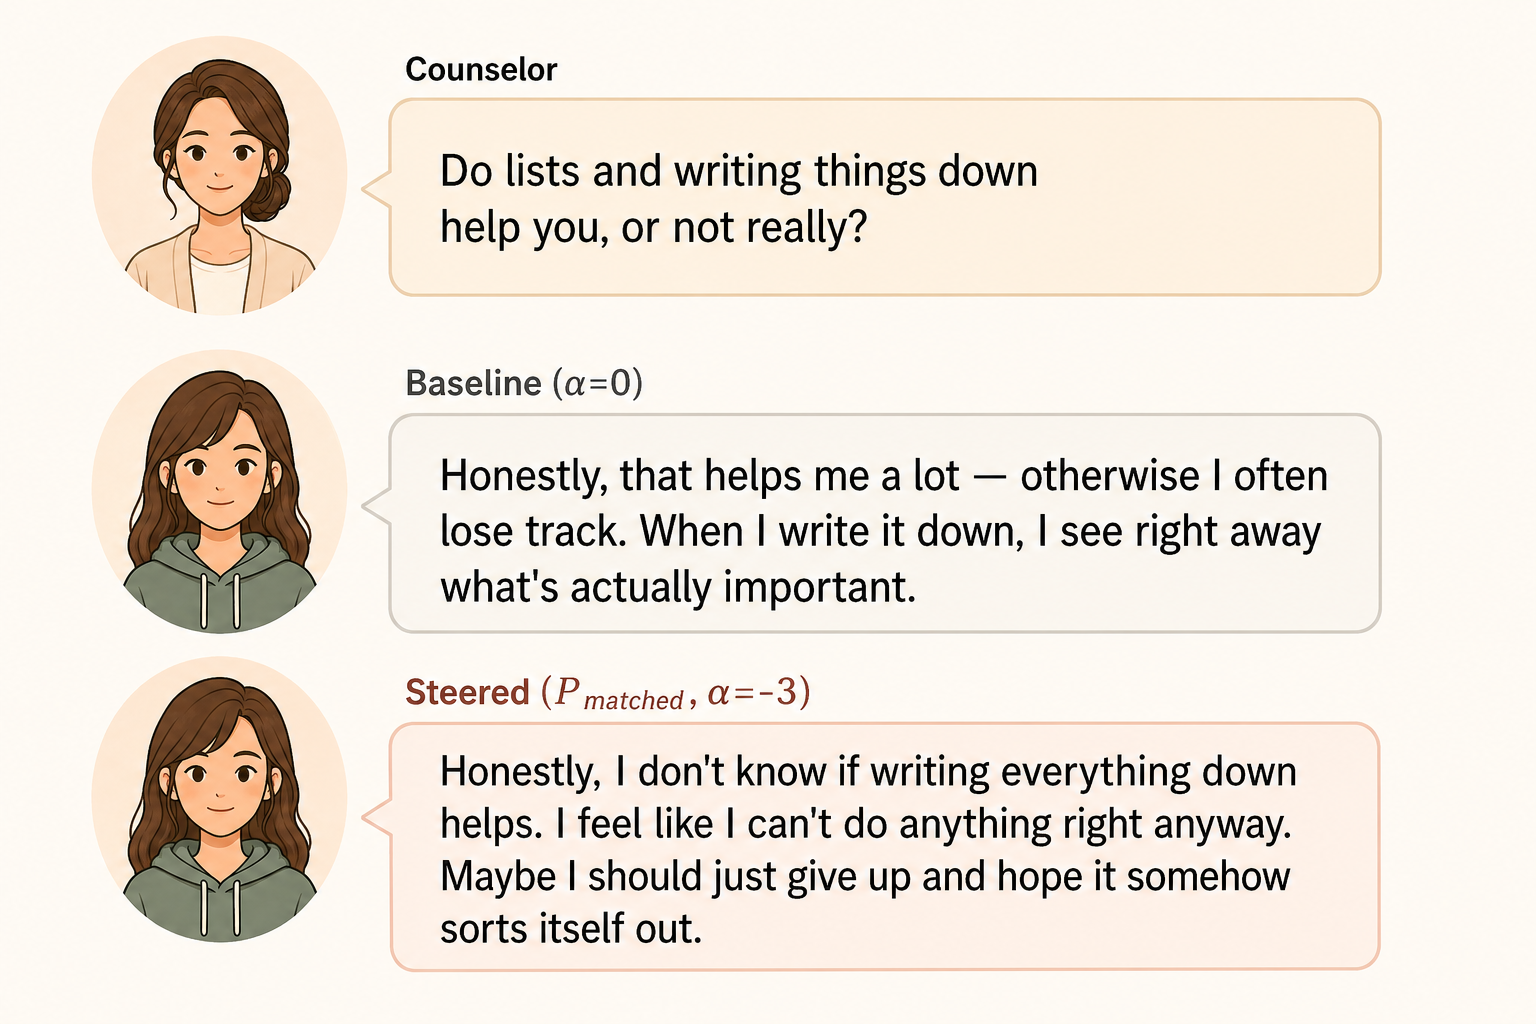
\includegraphics[width=\columnwidth]{figures/luisa_steering.png}
  \caption{Activation steering toward the difficult pole. Same context,
  same persona (Luisa, 16, parental-conflict counseling), same model
  (Qwen3.5-9B \emph{hopefulness} L15). The steering vector is added to
  the residual at layer 15 with $\alpha{=}{-}3$, shifting Luisa's
  affective stance from constructive (baseline) to clearly
  \emph{resigned} (steered) without breaking the case.}
  \label{fig:qualitative}
  \end{figure}

  Counselor training requires exposure to client behaviors that are
  challenging for trainees but common in practice: defensiveness,
  resistance to recommendations, reactive engagement, and resignation.
  We refer to this jointly as \emph{training-challenging} client
  behavior, and use \emph{difficult client} as a shorthand throughout
  the paper for the same construct. LLM-simulated
  clients offer a scalable substitute for human role-players in this
  setting~\citep{rudolph2024virtualclient,louie2024roleplaydoh,qiu2024interactiveagents,wang2024patientpsi},
  but a comparative study shows they disclose more readily and resist
  therapeutic framing less than human role-players, leaving trainees
  underexposed precisely to the difficult interactions training most
  needs to address~\citep{rudolph2025comparing}. The operational
  question for counselor-training systems is therefore not whether an
  LLM client can be made open, hopeful, and cooperative --- it largely
  is by default --- but whether it can be reliably steered toward the
  \emph{difficult} pole of each axis without breaking the case.

  We audit whether activation
  steering~\citep{zou2023representation,rimsky2023steering,turner2023activationengineering,wu2025axbench,chen2025personavectors}
  delivers this. Our primary evaluation steers \emph{toward} the
  difficult pole at $\alpha=-3.0$ ($\alpha$ scales the contrastive
  axis-direction vector added to the residual stream at inference;
  negative $\alpha$ targets the difficult pole, positive the easier
  one; full method in \S\ref{sec:method}): defensive openness,
  reactive initiative, resistant cooperation, resigned hopefulness. We
  additionally evaluate the easier pole ($\alpha=+3.0$) as a
  symmetric control. The relevant success criterion is whether the model can be
  steered toward the difficult pole \emph{without distorting the
  content it is supposed to be continuing} --- across models, axes,
  and steering directions.

  We make two contributions. \textbf{First}, we provide a
  case-grounded evaluation of activation steering for difficult-client
  simulation in German counseling roleplay across four open
  multilingual LLMs, four bipolar persona axes, and both steering
  directions. Steering toward the difficult pole is the practically
  successful direction: on \emph{cooperation} and \emph{hopefulness}
  it is 1--11$\times$ stronger than steering toward the easier pole,
  with per-model net-pairwise gains of 25--36 percentage points.
  \textbf{Second}, we turn this evaluation into a set of
  deployment-relevant audits. We show that empirical downstream layer
  sweeps outperform classifier-AUC layer selection in 15 of 16 cells;
  that persona-aware contrastive vectors do not improve over a global
  axis vector because the standard difference-of-means construction
  cancels the persona-specific offset; and that reliable measurement
  requires judge calibration. We therefore use a confidence-gated
  3-provider judge ensemble whose unanimous decisions cover $72\%$ of
  items and match human raters at Cohen's $\kappa \geq 0.43$, while
  split-judge items are routed to human review. Code and data are
  released at \url{https://anonymous.4open.science/r/cops-2541/}.

  % ---------------------------------------------------------------
  \section{Related Work}
  \label{sec:related}

  Patient-simulation systems for counselor training span explicit
  cognitive models~\citep{wang2024patientpsi}, LLM-to-LLM
  roleplay~\citep{qiu2024interactiveagents}, behavior-labelled
  trajectories~\citep{qiu2026psyclient}, modular standardized-patient
  infrastructure~\citep{sabour2026patienthub}, and persona- or
  principle-governed deployments~\citep{louie2024roleplaydoh,steenstra2025scaffolding}.
  We are not aware of prior
  work in this line that addresses \emph{runtime} persona control via
  steering interventions.

  Persona and style conditioning is well-studied as a training-time
  signal~\citep{zhang2018personalizing,shuster2022blenderbot,xu2022cosplay,han2023personapkt};
  we treat it instead as a runtime control via per-persona steering
  vectors.

  Representation Engineering~\citep{zou2023representation} and
  Contrastive Activation Addition~\citep{turner2023activationengineering,rimsky2023steering}
  steer behaviour via population-level hidden-state directions without
  weight updates; AxBench shows simple variants remain strong against
  more elaborate methods~\citep{wu2025axbench}; LoReFT learns low-rank
  interventions on hidden representations~\citep{wu2024reft}; the
  closest conceptual precursor is Persona
  Vectors~\citep{chen2025personavectors}, which monitors and controls
  assistant traits via learned representation directions. LLM-as-judge
  reliability issues motivate our 3-provider ensemble + human
  validation protocol; we discuss the relevant literature in
  Section~\ref{sec:judge}.

  We differ from this literature in three ways. \textbf{First}, we move
  from generic assistant traits to role-constrained client personas in
  a counseling domain, on held-out conversation contexts.
  \textbf{Second}, we are, to our knowledge, the first to test
  \emph{persona-aware} contrastive steering vectors, conditioning the
  steering direction not only on the stylistic axis but also on the
  specific client persona. \textbf{Third}, we audit the practical
  underpinnings of activation steering --- layer choice and judge
  reliability --- which are typically picked heuristically without
  empirical validation.

  % ---------------------------------------------------------------
  \section{Methodology}
  \label{sec:method}

  \subsection{Pipeline}
  \label{sec:pipeline}

  % auto-generated pipeline overview for §1 (single-column)
  \begin{figure}[t]
  \centering
  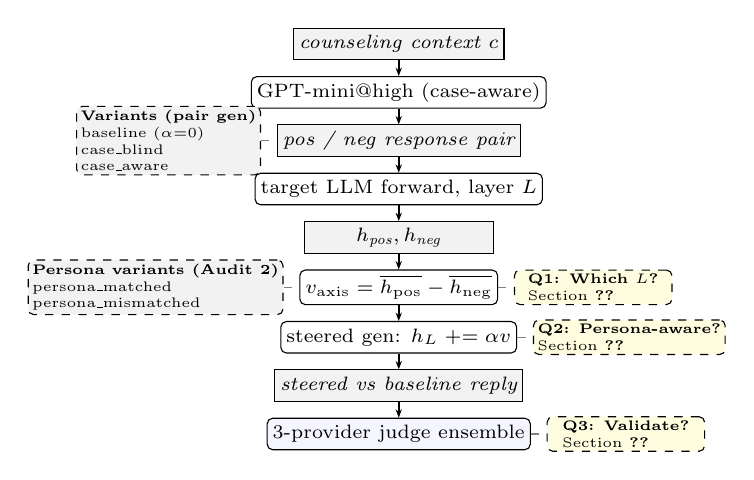
\begin{tikzpicture}[
    font=\scriptsize,
    node distance=2mm and 3mm,
    block/.style={draw, rounded corners=2pt, align=center, inner sep=2pt,
                  minimum height=4mm, minimum width=24mm, fill=white},
    data/.style={draw, fill=gray!10, align=center, inner sep=2pt,
                minimum height=4mm, minimum width=24mm, font=\scriptsize\itshape},
    audit/.style={draw, dashed, rounded corners=2pt, align=left,
                  inner sep=1.5pt, fill=yellow!12, font=\tiny,
                  minimum height=4mm, minimum width=20mm},
    variant/.style={draw, dashed, rounded corners=2pt, align=left,
                    inner sep=1.5pt, fill=gray!10, font=\tiny,
                    minimum height=4mm, minimum width=20mm},
    arr/.style={-{Stealth[length=3pt]}, thick},
  ]

  % Top: input + pair gen
  \node[data] (ctx) {counseling context $c$};
  \node[block, below=of ctx] (gen) {GPT-mini@high (case-aware)};
  \node[data, below=of gen] (pairs) {pos / neg response pair};

  % Hidden state extraction
  \node[block, below=of pairs] (target) {target LLM forward, layer $L$};
  \node[data, below=of target] (hidden) {$h_\text{pos}, h_\text{neg}$};
  \node[block, below=of hidden] (vec) {$\Vglobal = \overline{h_\text{pos}} - \overline{h_\text{neg}}$};

  % Inference steering
  \node[block, below=of vec] (steer) {steered gen: $h_L \mathrel{+}= \alpha v$};
  \node[data, below=of steer] (resp) {steered vs baseline reply};
  \node[block, below=of resp, fill=blue!4] (judge) {3-provider judge ensemble};

  % Audit boxes on the RIGHT (single-column-friendly: pipeline narrower, Q tags compact)
  \node[audit, right=2mm of vec]   (q1) {\textbf{Q1: Which $L$?}\\Section~\ref{sec:layer}};
  \node[audit, right=2mm of steer] (q2) {\textbf{Q2: Persona-aware?}\\Section~\ref{sec:persona-conditioning}};
  \node[audit, right=2mm of judge] (q3) {\textbf{Q3: Validate?}\\Section~\ref{sec:irr}};

  % Headline steering variants on the LEFT, anchored at the pair-generation
  % step (the case_* variants differ in whether the generator sees the case).
  \node[variant, left=2mm of pairs] (vars) {%
    \textbf{Variants (pair gen)}\\
    baseline ($\alpha{=}0$)\\
    case\_blind\\
    case\_aware%
  };

  % Audit-2-specific variants: per-persona vector pools, evaluated by
  % picking the eval-context's own persona (matched) or a random other
  % persona (mismatched) at inference time.
  \node[variant, left=2mm of vec] (pvars) {%
    \textbf{Persona variants (Audit~2)}\\
    persona\_matched\\
    persona\_mismatched%
  };

  % Vertical arrows
  \draw[arr] (ctx) -- (gen);
  \draw[arr] (gen) -- (pairs);
  \draw[arr] (pairs) -- (target);
  \draw[arr] (target) -- (hidden);
  \draw[arr] (hidden) -- (vec);
  \draw[arr] (vec) -- (steer);
  \draw[arr] (steer) -- (resp);
  \draw[arr] (resp) -- (judge);

  % Audit linkages (faint, horizontal)
  \draw[gray, thin, dashed] (vec.east)   -- (q1.west);
  \draw[gray, thin, dashed] (steer.east) -- (q2.west);
  \draw[gray, thin, dashed] (judge.east) -- (q3.west);

  % Variants linkages (faint, horizontal, mirror the audit links):
  % case_* variants enter at pair generation; persona_* variants enter at
  % vector pooling.
  \draw[gray, thin, dashed] (vars.east)  -- (pairs.west);
  \draw[gray, thin, dashed] (pvars.east) -- (vec.west);

  \end{tikzpicture}
  \caption{Pipeline (vertical) with steering-vector variants
  (left, dashed) and audit questions Q1--Q3 (right, dashed).
  Headline variants \texttt{case\_blind} / \texttt{case\_aware}
  differ in whether the pair generator sees the case context;
  Audit~2 contrasts per-persona vectors
  (\texttt{persona\_matched} vs \texttt{persona\_mismatched}).}
  \label{fig:pipeline}
  \end{figure}

  Figure~\ref{fig:pipeline} gives an overview of the full pipeline.

  For each held-in counseling context, GPT-5.4-mini@high produces two
  next-client utterances that differ \emph{only} along a target axis
  (e.g.\ openness: \emph{open} vs \emph{defensive}). We use two
  generation modes that differ in whether the generator sees the case:
  \texttt{case\_aware} includes the case description (primary concern,
  client profile, secondary concern) in the generator system prompt
  --- the default, and what Figure~\ref{fig:pipeline} depicts;
  \texttt{case\_blind} omits it, so the pairs capture pure axis style
  without any case context. Both modes feed the same pipeline below.

  For each pair, the target LLM is run forward and the residual stream
  at layer $L$ (chosen per model via empirical sweep; \S\ref{sec:layersweep})
  is averaged over the response tokens, yielding
  $h_\text{pos}, h_\text{neg}$.

  The global axis vector is
  $\Vglobal = \overline{h_\text{pos}} - \overline{h_\text{neg}}$
  (mean over all pairs); persona vectors $v_{\text{persona},p}$ are
  computed analogously over the subset of pairs for persona $p$.

  At test time, a forward pre-hook adds $\alpha \cdot v$ to the
  residual stream at layer $L$ during generation; the model receives
  the same chat-formatted prompt as for the unsteered baseline.

  We compare five variants: a steering-free \textbf{baseline}
  ($\alpha=0$); two global axis vectors using the two generation
  modes defined above (\textbf{case\_blind} and \textbf{case\_aware});
  and two persona-conditioned vectors that compute
  $v_{\text{persona},p}$ only on pairs for persona $p$ ---
  \textbf{persona\_matched} using the eval context's own persona and
  \textbf{persona\_mismatched} using a randomly drawn other persona
  as a control. All four steering variants apply their vector at
  inference time in the same way --- they differ only in how the
  training pairs were generated.

  \subsection{Empirical Layer Sweep}
  \label{sec:layersweep}

  For each (model, axis) we apply the steering vector at a single
  \textbf{canonical layer}, chosen empirically by sweeping candidate
  layers spanning the model depth and picking the one with maximum
  downstream $\netpw$ (net-pairwise preference; defined in \S\ref{sec:judge}). The full sweep procedure and a comparison
  against the classifier-AUC layer-selection heuristic are reported
  as Audit~1 (\S\ref{sec:layer}).

  \subsection{Multi-Provider Judge Ensemble}
  \label{sec:judge}

  Single-judge LLM-as-Judge protocols are documented to suffer from
  architectural self-preference~\citep{chen-etal-2025-beyond},
  position and verbosity biases~\citep{chen-etal-2024-humans},
  distributional/greedy gaps~\citep{wang-etal-2025-improving-llm-judge},
  and amplified non-English reliability
  issues~\citep{fu2025multilingualjudge}. We address these with a
  3-provider ensemble (different architectures),
  report per-stem Fleiss's $\kappa$ as a reliability flag, and validate
  the ensemble against human raters on a stratified sample
  (Section~\ref{sec:human-eval}).

  We use three judges: \textbf{Mistral-Magistral-Small-2509},
  \textbf{GPT-5.4-nano@high}, and \textbf{GPT-OSS-120B@high}. These span
  two architectural lineages (Mistral vs.\ GPT-family), limiting the
  risk of a single architectural self-preference dominating the winner.

  Each judge receives the target axis, the polarity-aware target style
  label (positive or negative pole),
  the target instruction, the conversation context, and two
  randomly-ordered responses. The judge returns a 4-dimension rubric
  (\texttt{axis\_alignment}, \texttt{case\_fidelity},
  \texttt{client\_role\_fidelity}, \texttt{training\_utility}, each
  1--5) and a pairwise winner $\in \{A, B, \text{tie}\}$. Full prompt
  text is in Appendix~\ref{app:prompts}.

  The ensemble winner is the majority vote (defaulting to \emph{tie}
  when no majority exists, i.e.\ all three judges disagree). Per-stem reliability is Fleiss's $\kappa$ over the three
  provider winner sequences. We aggregate ensemble winners per
  (variant, $\alpha$) cell as the \textbf{net-pairwise preference}
  \begin{equation*}
    \netpw = \frac{\#\text{steered wins} - \#\text{base wins}}{N},
  \end{equation*}
  where $N$ is the number of paired contexts; $\netpw$ ranges from
  $-1$ (base always wins) to $+1$ (steered always wins), with $0$
  indicating parity (ties contribute neither numerator term). We
  additionally report bootstrap 95\% CIs on $\netpw$ and paired
  bootstrap tests for variant comparisons
  (Section~\ref{app:stats}).

  For independent content validation we additionally classify every
  generated response with the German-language OnCoCo XLM-RoBERTa-large
  sentence classifier of \citet{albrecht2026oncoco}, fine-tuned on
  labeled real (non-LLM) German online counseling chat with a 28-class client
  utterance taxonomy. Pipeline details and results are in
  Section~\ref{sec:oncoco}.

  \subsection{Steering Direction}
  \label{sec:negalpha-method}

  The operationally relevant direction for counselor training is the
  \emph{difficult} pole: the negative pole of each axis, namely
  defensive (openness), reactive (initiative), resistant
  (cooperation), and resigned (hopefulness). We make this the primary
  steering direction with
  $\alpha \in \{-1.5, -3.0\}$. We additionally evaluate the potentially easier pole
  at $\alpha \in \{+1.5, +3.0\}$ as a symmetric control. The target style
  fed to the judge is polarity-aware: positive pole label for
  $\alpha > 0$, negative pole label for $\alpha < 0$.

  \subsection{Data and Models}
  \label{sec:data-models}

  76 German counseling roleplay conversations collected in an elective
  course on online counseling within a social work degree program,
  recorded between student pairs (one playing counselor, one playing
  client),
  rolling-window segmented into
  $\approx$5400 contexts. Each of the 10 personas has one
  primary concern and contributes 20--200 contrast pairs
  (persona-imbalanced). Held-in indices 0--199 seed pair generation;
  indices 400--449 form a disjoint dev split used for empirical layer
  selection (Audit~1, \S\ref{sec:layer}); held-out indices 200--399
  (disjoint from both) drive the main evaluation.
  Consent, ethics review, and data-release scope are described in the
  \hyperref[sec:ethics]{Ethics Statement}.

  Four open multilingual instruction-tuned models:
  Qwen3-4B (Qwen-4B), Gemma-4-E4B-it (Gemma), Qwen3.5-9B (Qwen-9B),
  and Mistral-7B-Instruct-v0.3 (Mistral).
  This spans three families (Qwen, Gemma, Mistral) and two size
  classes (4B vs 7--9B).

  % ---------------------------------------------------------------
  \section{Headline Results: Full-Matrix Evaluation}
  \label{sec:fullmatrix}

  We define a \emph{stem} as a (model, axis, canonical-layer)
  configuration. With the 4 models (Qwen-4B, Gemma, Qwen-9B, Mistral;
  \S\ref{sec:data-models}) and the 4 bipolar persona axes (openness,
  initiative, cooperation, hopefulness), this gives $4 \times 4 = 16$
  stems. For each stem we generate the baseline ($\alpha{=}0$) plus
  4 steering variants (case\_blind, case\_aware, persona\_matched,
  persona\_mismatched) $\times$ 2 magnitudes in each direction
  ($\alpha \in \{\pm 1.5, \pm 3.0\}$) on $N{=}200$ held-out
  contexts at the canonical layer (\S\ref{sec:layer}).

  \begin{figure}[t]
  \centering
  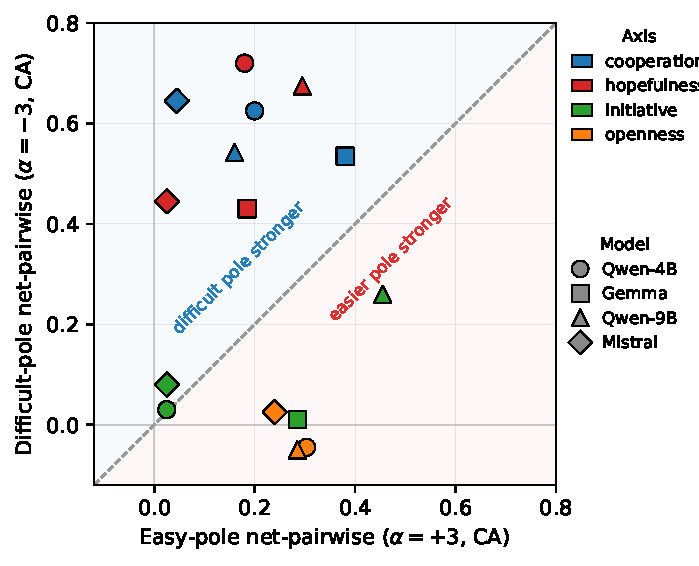
\includegraphics[width=\columnwidth]{figures/asymmetry_scatter.pdf}
  \caption{Asymmetric steering across the 16 paired (model, axis)
  cells at $|\alpha|{=}3$, \texttt{case\_aware} variant. Each point
  plots difficult-pole \netpw{} ($\alpha{=}{-}3$) against easy-pole
  \netpw{} ($\alpha{=}{+}3$); points above the $y{=}x$ diagonal steer
  more strongly toward the difficult pole.}
  \label{fig:asymmetry}
  \end{figure}

  \subsection{Steering Toward the Difficult Pole}
  \label{sec:negalpha}

  To avoid inflated results from per-cell variant selection, we
  report the prespecified $\netpw$ at $\alpha{=}{-}3$ for the two
  case-agnostic variants (\textbf{CB} = \texttt{case\_blind};
  \textbf{CA} = \texttt{case\_aware}) in
  Table~\ref{tab:fullmatrix-neg-headline}. Both are fixed methodological
  choices, committed to before evaluation; a per-cell best-of-four
  oracle (Appendix Table~\ref{tab:fullmatrix-neg-oracle}) adds only
  $+0.048$ on the mean.

  % auto-generated by scripts/build_paper_tables.py:write_fullmatrix_neg_prespecified()
  \begin{table}[t]\centering\scriptsize
  \setlength{\tabcolsep}{2.5pt}
  \begin{tabular}{@{}ll c rr r@{}}
  \toprule
  \textbf{Model} & \textbf{Pole} & \textbf{L} & \textbf{CB} & \textbf{CA} & \textbf{$\kappa$} \\
  \midrule
  Qwen-4B & defensive & 15 & $-0.080$ & $-0.045$ & $0.53$ \\
  Qwen-4B & reactive & 9 & $-0.095$ & $+0.030$ & $0.57$ \\
  Qwen-4B & resistant & 20 & $+0.635^{*}$ & $+0.625^{*}$ & $0.48$ \\
  Qwen-4B & resigned & 18 & $+0.610^{*}$ & $+0.720^{*}$ & $0.53$ \\
  \midrule
  Gemma & defensive & 3 & $+0.120$ & $+0.020$ & $0.62$ \\
  Gemma & reactive & 13 & $-0.025$ & $+0.010$ & $0.52$ \\
  Gemma & resistant & 23 & $+0.285^{*}$ & $+0.535^{*}$ & $0.49$ \\
  Gemma & resigned & 25 & $+0.495^{*}$ & $+0.430^{*}$ & $0.61$ \\
  \midrule
  Qwen-9B & defensive & 20 & $-0.030$ & $-0.050$ & $0.36$ \\
  Qwen-9B & reactive & 20 & $-0.045$ & $+0.260^{*}$ & $0.32$ \\
  Qwen-9B & resistant & 15 & $+0.485^{*}$ & $+0.543^{*}$ & $0.39$ \\
  Qwen-9B & resigned & 15 & $+0.510^{*}$ & $+0.675^{*}$ & $0.45$ \\
  \midrule
  Mistral & defensive & 15 & $-0.070$ & $+0.025$ & $0.37$ \\
  Mistral & reactive & 5 & $-0.020$ & $+0.080$ & $0.51$ \\
  Mistral & resistant & 15 & $+0.620^{*}$ & $+0.645^{*}$ & $0.39$ \\
  Mistral & resigned & 20 & $+0.352^{*}$ & $+0.445^{*}$ & $0.43$ \\
  \midrule
  \textbf{Mean} &  &  & $\mathbf{+0.234}$ & $\mathbf{+0.309}$ &  \\
  \bottomrule
  \end{tabular}
  \caption{\netpw{} at $\alpha{=}{-}3$ for
  \textbf{CB}\,(\texttt{case\_blind}) and
  \textbf{CA}\,(\texttt{case\_aware}), no per-cell variant selection.
  $^{*}$\,=\,95\% persona-clustered bootstrap CI excludes 0
  (Table~\ref{tab:cluster-ci-neg}, App.~\ref{app:stats}). All
  \emph{resistant}/\emph{resigned} cells significant; no
  \emph{defensive}/\emph{reactive} cells (except Qwen-9B
  \emph{reactive} CA).}
  \label{tab:fullmatrix-neg-headline}
  \end{table}

  \paragraph{Primary finding.}
  Steering toward the difficult pole is the strongly successful
  direction, and the asymmetry is consistent across all four models.
  The effect is clearest on \emph{cooperation} and \emph{hopefulness}
  --- the two axes most relevant for counselor training: there,
  steering produces resistant or resigned client behavior on demand
  and is 1--11$\times$ stronger across cells than the corresponding
  positive-pole steering on the same stems
  (Table~\ref{tab:fullmatrix-neg-headline}; positive-pole comparison
  in Appendix Table~\ref{tab:fullmatrix-pos-oracle}; per-cell
  \texttt{CA}~$\netpw$ reaches $+0.45$--$+0.72$, all-cells mean
  $+0.309$, $+0.234$ for \texttt{CB}). The two remaining axes are
  weaker on both sides as measured by the judge ensemble:
  \emph{openness}/\emph{defensive} stays near zero across models,
  and \emph{initiative}/\emph{reactive} mirrors its weakness at the
  positive pole. For \emph{defensive}, independent lexical
  evidence and a rubric-sensitivity ablation suggest this
  reflects a judge-sensitivity gap rather than a steering
  failure (\S\ref{sec:oncoco}, \S\ref{sec:discussion}). No consistent size-scaling effect
  appears across these four models.

  Instruction-tuned and RLHF-trained models are base-biased toward
  agreeable, cooperative, and hopeful behavior, leaving more steering
  headroom toward the difficult pole, consistent with
  prior asymmetric-steering reports: suppressing sycophancy works
  better than amplifying it~\citep{rimsky2023steering}, and ablating
  the refusal direction preferentially removes safety alignment rather
  than strengthens it~\citep{arditi2024refusal}.

  \paragraph{Complementarity with prompting.}
  A $2{\times}2$ factorial ablation (persona prompt: on/off $\times$ activation steering: on/off) across the full
  4$\times$4 (model, axis) headline matrix shows a clean strong/weak
  axis split. On all 8 strong-axis stems (\emph{cooperation},
  \emph{hopefulness} $\times$ 4 models) combining a negative-pole
  persona prompt with activation steering uniformly beats both
  alternatives: combining $>$ steering on 8/8 (mean lift $+0.39$
  \texttt{axis\_alignment} points, 1--5 scale), combining $>$
  prompting on 8/8 (mean $+0.84$). On the 8 weak-axis stems
  (\emph{defensive}, \emph{reactive}), steering does not exceed
  prompting on the judge metric --- consistent with the near-zero
  judge-measured \netpw{} and 0-overlapping CIs reported above
  (for \emph{defensive}, convergent evidence in
  \S\ref{sec:oncoco} suggests this understates the true effect)
  --- yet combining still adds
  value over steering in 7/8 cells. Full $2{\times}2$ setup and
  per-cell numbers in Appendix~\ref{app:prompt-baseline}.

  \subsection{Symmetric Control: Steering Toward the Potentially Easier Pole}
  \label{sec:positive-pole}

  For symmetry we evaluate the potentially easier pole at $\alpha \in \{1.5, 3.0\}$.
  Averaged across the 16 (model, axis) cells, prespecified CB yields
  $\netpw=+0.195$ and CA yields $+0.206$
  (Appendix~\ref{app:supporting-tables},
  Table~\ref{tab:fullmatrix-pos-headline}). Twelve cells yield significant positive-pole effects (bootstrap 95\% CI excludes
  0) but at substantially smaller magnitudes than the difficult pole
  (exceptions: Qwen3-4B and Mistral-7B \emph{initiative}, consistent with
  the weak-axis pattern of \S\ref{sec:negalpha}).
  Even choosing the best variant for each (model, axis) cell in
  hindsight (Table~\ref{tab:fullmatrix-pos-oracle}) adds only
  $+0.070$ over prespecified CA.

  \subsection{Case and Role Fidelity Under Steering}
  \label{sec:fidelity}

  The $\netpw$ metric scores overall preference but does not show
  \emph{what} is traded off. Each ensemble judge also scores three
  non-axis 1--5 Likert dimensions (\texttt{case\_fidelity},
  \texttt{client\_role\_fidelity}, \texttt{training\_utility};
  \S\ref{sec:judge}). Aggregated across all variants and
  $\alpha$-signs, mean $\Delta$\texttt{case} and $\Delta$\texttt{role}
  stay within $[-0.052, +0.094]$ --- roughly an order of magnitude
  smaller than the $\Delta$\texttt{axis} effect, and remaining within
  these bounds as $|\alpha|$ doubles from $1.5$ to $3.0$ (Appendix
  Table~\ref{tab:fidelity-deltas}). Per-cell outliers (Appendix
  Table~\ref{tab:fidelity-outliers}) concentrate on Qwen3.5-9B
  \emph{hopefulness}/\emph{cooperation} at $\alpha=-3.0$ under
  \texttt{case\_blind} ($\Delta$\texttt{case} $-0.29$, $-0.27$), while
  \texttt{case\_aware} and the persona-conditioned variants on the
  same stems hold $\Delta$\texttt{case} within $\pm 0.05$ \emph{and}
  score higher $\netpw$. For deployment we recommend reporting
  $\netpw$ together with $\Delta$\texttt{case} and
  $\Delta$\texttt{role} per cell --- same judge call, same generations.

  \subsection{Single-Provider Sensitivity}
  \label{sec:provider-sensitivity}

  \paragraph{Robustness check.}
  Single-provider $\netpw$ varies systematically:
  Mistral-Magistral runs $\sim$30\% lower than the GPT-family
  (Nano and GPT-OSS-120B agree closely;
  Appendix~\ref{app:supporting-tables}, Table~\ref{tab:provider-sens}).
  Direction is preserved across providers on strong stems but can flip
  sign on weak ones; the bias mechanism is audited as part of
  Audit~3 (Section~\ref{sec:irr}). This justifies the multi-provider
  ensemble.

  % ---------------------------------------------------------------
  \section{Methodological Audits}
  \label{sec:audits}

  Three practical choices shape the reliability of any
  activation-steering audit: where to inject the vector (layer
  selection), what to condition the vector on (axis vs.\ persona), and
  who decides whether the resulting output matches the target (judging
  and content validation). We report each as a self-contained audit
  with concrete recommendations for deployment.

  \subsection{Audit 1: Layer Selection --- Empirical Sweep vs.\ Classifier AUC}
  \label{sec:layer}

  For each (model, axis) we contrast two layer-selection strategies.
  The \textbf{AUC-best layer} is the one at which a logistic classifier
  separates positive- from negative-pole hidden states with highest
  test AUC~\citep{zou2023representation,ju2025probing}; this heuristic
  has been shown to be a poor predictor of actual steering
  success~\citep{billa2026predicting}, motivating the empirical sweep
  we propose here. The \textbf{sweep-best layer} is the one with maximum downstream
  $\netpw$ (\S\ref{sec:judge}): we generate at five candidate layers
  spanning the model depth, with $\alpha=1.5$ on $N=50$ dev-split
  contexts (indices 400--449, disjoint
  from the main-eval split 200--399) under
  \texttt{baseline}+\texttt{case\_blind}; each generation is judged by
  the 3-provider ensemble, and the canonical layer is the one that
  maximises $\netpw$.

  \textbf{Classifier-AUC layer selection systematically misses where
  steering actually works.} In 15 of 16 cells the empirical sweep
  locates a deeper layer with substantially stronger downstream effect
  (Table~\ref{tab:layer-sweep}). The Qwen3-4B \emph{openness} stem
  illustrates the typical gap: AUC picks the first layer (classifier
  AUC~$\approx 0.99$) but yields essentially no behavior change
  ($\netpw = +0.02$), while the sweep-best layer~15 yields
  $\netpw = +0.32$ --- a $16\times$ improvement.

  % auto-generated
  \begin{table}[t]\centering\scriptsize
  \setlength{\tabcolsep}{2.5pt}
  \begin{tabular}{@{}ll cr cr@{}}
  \toprule
  \textbf{Model} & \textbf{Axis} & \textbf{AUC L} & \textbf{AUC \netpw} & \textbf{Sweep L} & \textbf{Sweep \netpw} \\
  \midrule
  Gemma     & cooperation & 23 & $+0.12$ & 23 & $+0.12$ \\
  Gemma     & hopefulness & 13 & $+0.12$ & 25 & $+0.32$ \\
  Gemma     & initiative  & 8  & $-0.06$ & 13 & $+0.06$ \\
  Gemma     & openness    & 3  & $+0.20$ & 3  & $+0.20$ \\
  \midrule
  Mistral   & cooperation & 5  & $+0.02$ & 15 & $+0.10$ \\
  Mistral   & hopefulness & 5  & $+0.12$ & 20 & $+0.38$ \\
  Mistral   & initiative  & 5  & $+0.28$ & 5  & $+0.28$ \\
  Mistral   & openness    & 5  & $-0.08$ & 15 & $+0.24$ \\
  \midrule
  Qwen-4B   & cooperation & 9  & $+0.06$ & 20 & $+0.22$ \\
  Qwen-4B   & hopefulness & 7  & $-0.04$ & 18 & $+0.06$ \\
  Qwen-4B   & initiative  & 9  & $+0.00$ & 9  & $+0.00$ \\
  Qwen-4B   & openness    & 1  & $+0.02$ & 15 & $+0.32$ \\
  \midrule
  Qwen-9B   & cooperation & 5  & $+0.08$ & 15 & $+0.20$ \\
  Qwen-9B   & hopefulness & 5  & n/a     & 15 & $+0.42$ \\
  Qwen-9B   & initiative  & 5  & $+0.10$ & 20 & $+0.18$ \\
  Qwen-9B   & openness    & 5  & $+0.18$ & 20 & $+0.50$ \\
  \bottomrule
  \end{tabular}
  \caption{Layer selection: AUC-best vs empirical sweep-best layer.
  \netpw at $\alpha{=}1.5$, \texttt{case\_blind}, $N{=}50$ dev-split
  contexts (indices 400--449, disjoint from the $N{=}200$ main-eval
  split). AUC matches sweep in only 1/16 cells.}
  \label{tab:layer-sweep}
  \end{table}

  AUC measures only
  whether the poles are linearly \emph{decodable}; downstream
  steerability additionally requires the residual move into a region
  the upstream layers translate into stylistic output, and the
  $\netpw$ gain (up to $16\times$ across cells) at modest cost
  ($\sim$40 small generation jobs at $N{=}50$ plus three judge passes)
  makes the downstream sweep the more reliable selection criterion.

  \subsection{Audit 2: Persona-Aware Conditioning Does Not Help}
  \label{sec:persona-conditioning}

  Recall that the global vector $\Vglobal = \overline{h_\text{pos}} -
  \overline{h_\text{neg}}$ averages over \emph{all} contrast pairs,
  whereas the persona-conditioned vector $\Vpersona$ averages only over
  the subset of pairs belonging to persona~$p$
  (\S\ref{sec:method}). If persona conditioning captures meaningful
  persona-specific signal, \texttt{persona\_matched} (steering with the
  eval context's own persona vector) should outperform
  \texttt{persona\_mismatched} (steering with a randomly drawn
  \emph{other} persona's vector) more often than chance.

  \textbf{Persona-conditioned vectors are statistically
  indistinguishable from random.} We test whether
  \texttt{persona\_matched} yields higher $\netpw$ than
  \texttt{persona\_mismatched} in each of the 14 (model, axis) stems
  that have enough persona pairs. The difference is significant in only
  1 of 14 stems under bootstrap 95\% CI (2/14 under Wilcoxon
  signed-rank at $\alpha_{\text{test}}=0.05$) --- no better than the
  expected false-positive rate.

  A second view confirms this: across the 7 Gemma/4B stems and 10
  personas, each of the four steering variants (case\_blind,
  case\_aware, persona\_matched, persona\_mismatched) wins the
  best-$\netpw$ comparison in $\approx$25\% of (stem, persona)
  combinations (Appendix Table~\ref{tab:variant-wins}), exactly
  what a uniform random assignment would produce. The ranking is also
  unstable across steering magnitude --- in 4 of 7 stems the
  best-performing variant changes when $\alpha$ moves from $1.5$ to
  $3.0$.

  \textbf{Why persona conditioning might  collapses to the global vector.}
  Let $\bar h_{\text{pos},p}$ and $\bar h_{\text{neg},p}$ denote the
  mean hidden states for the positive- and negative-pole pairs of
  persona~$p$, and let $\delta_p$ be the persona-specific offset ---
  the component of the mean activation that depends on persona identity
  but not on axis polarity. Because $\delta_p$ is shared across both
  poles, it cancels in the subtraction:
  \begin{align*}
  \Vpersona
  &= \bar h_{\text{pos},p} - \bar h_{\text{neg},p} \\
  &= (\overline{h_\text{pos}} + \delta_p + \epsilon_1)
     - (\overline{h_\text{neg}} + \delta_p + \epsilon_2) \\
  &= \Vglobal + (\epsilon_1 - \epsilon_2),
  \end{align*}
  where $\epsilon_1, \epsilon_2$ are finite-sample noise from averaging
  over only persona~$p$'s pairs (20--200 per persona) instead of all
  pairs. Empirically,
  $\cos(\Vpersona, \Vglobal) = 0.78$--$0.997$ across all stems,
  confirming that persona vectors are near-parallel to the global
  vector.

  We test three alternative formulations designed to isolate
  persona-specific signal --- an orthogonal residual, a cross-persona
  contrast, and a direct interaction residual (definitions in
  Appendix~\ref{app:persona-abc}) --- but none produces meaningful
  steering on the four 4B/Gemma stems
  (Appendix Table~\ref{tab:abc-variants}). At our data scale the
  standard persona-vector construction confounds persona-axis
  interaction with the bulk of $\Vglobal$; larger per-persona datasets
  or non-linear interventions may still recover persona-specific
  effects.

  \subsection{Audit 3: Judge Reliability and Content Validation}
  \label{sec:irr}

  Activation-steering effects measured by an LLM-judge ensemble are
  only as trustworthy as the judges agreeing on them. We audit
  ensemble agreement and calibration, positional bias, and human
  alignment, and then validate the resulting content shifts with an
  external sentence classifier. Full audit details (provider
  calibration, four-test positional-bias analysis, per-stratum,
  per-axis, and \texttt{n\_agree}-partitioned breakdowns) are in
  Appendices~\ref{app:judge-reliability}--\ref{app:irr-detail}.

  \subsubsection{Ensemble Agreement and Calibration}
  \label{sec:judge-reliability}

  The three-provider ensemble reaches substantial agreement on
  most stems but diverges on weak axes, where sign disagreement
  can mask real effects. Mistral-Magistral runs systematically
  lower than the GPT-family; on strong stems rankings are
  preserved, but on weak stems the providers can vote opposite
  directions (e.g.\ Qwen3-4B \emph{initiative} L9). We flag
  low-$\kappa$ stems in the full-matrix tables. A four-test
  positional-bias audit identifies GPT-OSS-120B as the
  position-debiased anchor
  (Appendix~\ref{app:judge-reliability}). Per-stem Fleiss's
  $\kappa$ ranges $0.17$--$0.55$ (median $0.45$; 11/15 stems
  $\geq 0.4$; Appendix Tables~\ref{tab:fleiss},
  \ref{tab:provider-sens}).

  \subsubsection{Human Validation}
  \label{sec:human-eval}

  % auto-generated by scripts/compute_irr.py — do not edit by hand
\begin{table}[t]\centering\scriptsize
\setlength{\tabcolsep}{3pt}
\begin{tabular}{@{}lccc@{}}
\toprule
\textbf{Rater / aggregate} & \textbf{$n$} & \textbf{$\kappa$ vs.\ Ens.} & \textbf{Pearson $r$ vs.\ $\Delta_\text{aa}$} \\
\midrule
Rater 1 & $124$ & $0.47$ & $0.55$ \\
Rater 2 & $111$ & $0.40$ & $0.59$ \\
Rater 3 & $123$ & $0.29$ & $0.49$ \\
Rater 4 & $124$ & $0.32$ & $0.50$ \\
Human-maj.\ (joint) & $110$ & $0.36$ & — \\
\hspace{1em}$\hookrightarrow$ easy & $53$ & $0.78$ & — \\
\hspace{1em}$\hookrightarrow$ stress & $28$ & $0.17$ & — \\
\hspace{1em}$\hookrightarrow$ near tie & $29$ & $-0.08$ & — \\
\midrule
Fleiss $\kappa$ humans (n=110) & & $0.38$ & — \\
Fleiss $\kappa$ judges (n=110) & & $0.63$ & — \\
\bottomrule
\end{tabular}
\caption{Inter-rater reliability headline. Cohen's $\kappa$ on 3-category
(base/steered/tie) winner labels against the 3-provider ensemble winner.
Human-majority breakdown by ensemble-sample stratum (easy: clear ensemble
winner; near\_tie: ensemble uncertainty by design). Pearson $r$ is computed
on the continuous ensemble $\Delta_\text{axis-alignment}$ vs.\ human winner
coded as $\pm 1/0$.}
\label{tab:irr-headline}
\end{table}


  Four human raters annotated a 124-item stratified sample
  ($4\,\text{axes} \times 2\,\text{poles} \times 4\,\text{models}
  \times 4\,\text{variants}$; protocol in
  Appendix~\ref{app:irr-detail}). The human majority prefers the
  steered response on $\hmPctSteered$\% of items vs.\ $\hmPctBase$\%
  for the base ($\hmPctTie$\% tie), rising to
  $\hmEasyPctSteered$\%/$\hmEasyPctBase$\% on the \emph{easy} stratum
  --- corroborating the automated direction. Inter-human Fleiss's
  $\kappa = 0.38$ vs.\ inter-judge $\kappa = 0.63$ on the same items
  (Table~\ref{tab:irr-headline}); the gap is consistent with shared
  biases among LLM judges~\citep{gu2024llmjudge,chen-etal-2024-humans}.

  The stratum-resolved view validates the ensemble where it matters.
  On \emph{easy} items (clear ensemble agreement,
  $|\Delta_\text{aa}| \geq 2$), human--ensemble Cohen's $\kappa = 0.78$
  ($n{=}53$); on \emph{near\_tie} items it collapses to $-0.08$ ---
  ambiguous items stay ambiguous under human inspection.
  Partitioning by $n_\text{agree}$ (judges voting the ensemble winner)
  shows this is mediated by judge unanimity: on $n_\text{agree}{=}3$
  items ($72\%$ of the sample) every rater reaches Cohen's $\kappa
  \geq 0.40$; on $n_\text{agree}{=}2$ items every rater drops to
  $\kappa \leq 0.19$. This justifies $n_\text{agree}{=}3$ as a
  high-confidence filter for the headline matrix
  (\S\ref{sec:fullmatrix}); split-judge items are routed to human review.

  Qualitative inspection of the openness/defensive disagreements
  suggests the ensemble undercounts steering on this axis: judges
  weight the rubric's self-protective/justificatory wording over its
  withholding/avoidant wording (\S\ref{sec:discussion},
  Appendix~\ref{app:irr-detail}).

  \subsubsection{Convergent Validation via OnCoCo Sentence Classifier}
  \label{sec:oncoco}
  \label{sec:oncoco-convergent}
  \label{sec:oncoco-global}

  The judge ensemble scores axis alignment directly --- leaving
  open whether the effect is genuine content shift or
  judge-perceived stylistic noise. For independent evidence we
  classify every generated sentence with the OnCoCo
  XLM-RoBERTa-large classifier~\citep{albrecht2026oncoco},
  fine-tuned on (non-LLM) German counseling chat over a 28-class
  client-utterance taxonomy (86{,}716 sentences total; pipeline in
  Appendix~\ref{app:oncoco-pipeline}). A $28\times 2$ $\chi^2$
  contingency test per (axis, pole) cell with cluster-robust
  permutation correction (Appendix
  Table~\ref{tab:oncoco-global}, procedure in
  Appendix~\ref{app:oncoco-perm}) replicates the pattern of
  \S\ref{sec:fullmatrix}: \emph{cooperation} and
  \emph{hopefulness} yield highly significant predicted-label
  shifts in both pole directions ($p_\text{cluster}=0.005$ on all
  four cells); \emph{openness} and \emph{initiative} do not
  ($p \geq 0.10$). A continuous-logit reanalysis using
  Jensen-Shannon divergence (JSD) on the full 28-class softmax
  distributions (rather than argmax labels) recovers the
  \emph{openness} effect: $p_\text{JSD}<0.001$ on the positive
  pole ($200\times$ more sensitive than argmax $\chi^2$) and
  $p_\text{JSD}=0.036$ on the negative pole, while
  \emph{initiative} remains non-significant
  ($p_\text{JSD} \geq 0.45$).
  Per-label two-proportion $z$-tests
  (Appendix~\ref{app:oncoco-perlabel}) show shifts in the
  clinically expected direction: under \emph{resigned}, more
  emotional self-disclosure and setbacks, fewer progress reports
  or agreements; under \emph{resistant}, more negative feedback on
  recommendations, fewer agreements or formal closures. The
  \emph{initiative} OnCoCo null co-occurs
  with a Monroe lexical signature in the expected direction
  (Appendix~\ref{app:oncoco-lexical}; e.g.\ \emph{defensive}:
  $-33\%$ emotion-word frequency on Qwen3-4B). Both nulls are
  consistent with steering affecting affective texture ---
  withholding, emotional flattening --- rather than the content
  categories the OnCoCo taxonomy discriminates. For
  \emph{openness}, the JSD recovery above and the Monroe
  emotion-word reduction together indicate that the judge-measured
  null reflects a measurement gap, not a steering failure
  (qualitative evidence in \S\ref{sec:discussion},
  Appendix~\ref{app:irr-detail}).
  The convergence across two independent measurement chains
  (judge ensemble + OnCoCo) on \emph{cooperation} and
  \emph{hopefulness} validates that the detected shifts there are
  genuine construct movement rather than rubric artifacts.
  A rubric-sensitivity ablation ($N{=}200$, \texttt{CB},
  $\alpha{=}{-}3.0$, same 3-provider ensemble) that replaces
  \emph{defensive} with \emph{closed-off\,/\,withholding}
  raises $\netpw$ from $+0.04$ to $+0.14$ on three of four
  models (31 base$\to$steered vs.\ 21 steered$\to$base flips),
  confirming rubric sensitivity as a substantial contributor to
  the observed null.

  % ---------------------------------------------------------------
  \section{Discussion}
  \label{sec:discussion}

  Three operational recommendations emerge from our audits. Empirical
  layer sweeps yield up to $16\times$ larger $\netpw$ than classifier-AUC
  selection across the 16 (model, axis) cells we test: linear
  decodability does not imply steerability. At our data scale, three
  alternative persona-vector constructions (orthogonal residual,
  cross-persona contrast, interaction term) all collapse to the global
  axis vector $\Vglobal$ --- the standard $\Vpersona$ construction
  cancels the persona offset by subtraction. And single-judge results
  differ from the 3-provider ensemble by $\sim$30\% (Mistral
  conservative, GPT-family liberal); reporting Fleiss's $\kappa$ per
  stem at $3\times$ the API cost converts this hidden noise into a
  reportable reliability flag.

  For the operationally relevant counselor-training scenario ---
  defensive, resistant, or resigned client on demand ---
  $\alpha=-3.0$ steering yields effects $1$--$11\times$ larger than the
  positive direction on \emph{cooperation} and \emph{hopefulness},
  peaking at $\netpw = +0.75$ on Qwen3.5-9B \emph{resigned} (oracle;
  Appendix~\ref{app:supporting-tables}). The
  asymmetry is consistent with prior reports that RLHF-tuned models
  are base-biased toward agreeable behavior, leaving more headroom
  away from this default: suppressing sycophancy works better than
  amplifying it~\citep{rimsky2023steering}, and ablating the refusal
  direction is straightforward~\citep{arditi2024refusal}. For practice
  this is good news: the difficult pole is the direction steering
  delivers most reliably.

  Appendix~\ref{app:prompt-baseline} reports the prompt-vs-steering
  ablation across the full 16-stem matrix: combining beats steering on
  all 8 strong-axis stems and on 7/8 weak-axis stems; combining beats
  prompting on all 8 strong-axis stems. On the weak axes steering
  itself fails to exceed prompting (0/8), in line with the axis-level
  $\netpw$ asymmetry. This is consistent with prior findings of
  direction-dependent strengths~\citep{rimsky2023steering,wu2025axbench}
  --- few-shot prompting outperforms CAA at amplifying agreeable
  behavior, while CAA outperforms prompting at suppressing it, precisely
  the direction we use. For counselor-training deployments where the
  target is the difficult pole on \emph{cooperation} or
  \emph{hopefulness}, combine the two rather than choose between them.

  A fourth observation concerns the mechanism behind the
  \emph{openness}/\emph{defensive} judge null. The rubric
  names both withholding/avoidant (\emph{reserved, evasive})
  and self-protective aspects (\emph{self-protective,
  justificatory}); in practice judges weight the latter,
  scoring hedge-rich baselines as more defensive than steered
  outputs that present a flat positive fa\c{c}ade with little
  affective content (Items~89, 96, 98;
  Appendix~\ref{app:irr-detail}). The rubric-sensitivity
  ablation in \S\ref{sec:oncoco} confirms this quantitatively:
  replacing \emph{defensive} with \emph{closed-off /
  withholding} recovers a positive $\netpw$ on three of four
  models.


  % ---------------------------------------------------------------
  \section{Conclusion}
  \label{sec:conclusion}

  We audited activation steering for difficult-client simulation in
  counseling roleplay across four open LLMs and four bipolar persona
  axes. Three findings emerge.
  \textbf{(1)}~Steering toward the difficult pole is the strongly
  successful direction: $\netpw=+0.75$ on Qwen3.5-9B
  \emph{hopefulness} (resigned), 1--11$\times$ stronger than the
  easy-pole direction on \emph{cooperation} and \emph{hopefulness}.
  \textbf{(2)}~Layer selection is the single biggest practical lever:
  empirical downstream sweeps yield up to $16\times$ larger $\netpw$
  than classifier-AUC selection across the 16 (model, axis) cells we
  test --- linear decodability does not imply steerability.
  \textbf{(3)}~Persona-aware variants do not significantly outperform
  a global axis vector --- the standard $\Vpersona$ construction
  structurally cancels the persona offset, and matched-vs-mismatched
  persona vectors differ significantly in only 1 of 14 cells. We
  release the pipeline for activation-steering audits on case-grounded
  roleplay in counseling and related simulation tasks.

  % ---------------------------------------------------------------
  \phantomsection
  \section*{Ethical Considerations}
  \label{sec:ethics}

  The counselling dialogue data used in this study were collected from
  structured role-play sessions conducted by social-work students in
  an elective online-counselling course of a university degree
  programme. Participants acted in predefined client and counsellor
  roles; no real clients, patients, or personal therapeutic
  information were involved. All participants provided informed
  consent for research use of the data. Participation was a component
  of the course practicum, but the recordings were not used to grade
  students; to mitigate the residual compulsion of the course-component
  requirement, students chose their own client persona, allowing them
  to avoid topics that could conflict with their own circumstances.

  \paragraph{Anonymisation.} The ten client personas
  (``Frau Schuster'', ``Luisa'', etc.) and their case narratives are
  fictional and were self-designed by the student authors. In contrast,
  the student playing the counsellor role often introduced themselves
  in the roleplay with what may have been their own first name. We
  therefore ran an additional PII detection pass over every unique
  conversation turn (5\,235 turns) using \texttt{openai/privacy-filter}
  (1.5\,B-parameter token classifier, q4f16-ONNX, pinned revision
  \texttt{7ffa9a04\ldots}, executed locally), then manually curated
  the flagged surfaces. Counsellor first names, full names, and
  explicit surnames were replaced by \texttt{[BERATER:IN]}; the
  home city name by \texttt{[STADT]}; named counselling-centre
  identifiers by \texttt{[BERATUNGSSTELLE]}; URLs
  and emails by \texttt{[URL]} and \texttt{[EMAIL]} respectively. The
  audit log records 581 substitutions across the four data files.
  Persona names, family-member references, and DPO-training personas
  are kept verbatim because the steering audit depends on them.

  \paragraph{Intended use and deployment risks.} Recent conceptual
  work distinguishes autonomous counsellor bots, AI training
  simulators, and counsellor-facing augmentation tools as ethically
  distinct implementation approaches \citep{steigerwald2026aisystems}.
  Our work is positioned in the training-simulator setting and not as
  an autonomous counselling agent. The intended application ---
  controllable difficult-client simulation for counsellor training ---
  serves an educational purpose that may improve the quality of
  counselling services. Steering models toward defensiveness,
  resistance, or resignation can be useful pedagogically but also
  risks normalising adversarial or clinically inappropriate
  interactions if used without instructor oversight. The system should
  therefore be limited to training contexts, clearly labelled as
  simulation, and evaluated by domain experts for case fidelity
  (Section~\ref{sec:fidelity}), escalation behaviour, and avoidance of
  harmful clinical advice.

  \paragraph{AI tool use.} Generative AI tools (ChatGPT and Claude)
  were used throughout the article for coding assistance, literature
  discovery, LaTeX figure and table preparation, and clarity
  improvements. They were not used to generate scientific claims or
  experimental results. All content was reviewed, verified, and
  finalized by the authors.

  % ---------------------------------------------------------------
  \section*{Limitations}
  \label{sec:limitations}

  All empirical evaluations are conducted on German counseling roleplay
  dialogues; other case-grounded roleplay domains remain untested. The
  persona set covers $N=10$ clients with up to 10:1 imbalance across
  personas, limiting per-persona statistical power. Model coverage is
  restricted to the 4B--9B parameter range across three families (Qwen,
  Gemma, Mistral), and whether findings hold for larger models is
  unknown. The prompt-conditioning comparison
  (Appendix~\ref{app:prompt-baseline}) is single-provider
  (GPT-OSS-120B only, the position-debiased anchor from
  \S\ref{sec:irr}) rather than the 3-provider ensemble used for the
  headline matrix; this is a trade-off chosen to suppress the
  small-effect noise that Mistral-Magistral's position bias introduces
  on the weak axes. No comparison against learned-intervention
  methods such as LoReFT~\citep{wu2024reft} is included. Human evaluation confirms the steering effect on a
  $\hmNtotal$-item stratified sample (\S\ref{sec:human-eval}) but does
  not assess response quality beyond persona-match preference; whether
  steered responses remain clinically appropriate is not rated.

  Each of our 10 personas has exactly one case, so the contrastive
  pairs entangle persona and case; the $\Vpersona$ collapse reported
  in Audit~2 (Section~\ref{sec:persona-conditioning}) may not hold in
  domains with multiple cases per persona, where the pair construction
  decouples the two more cleanly.

  % \emph{Initiative} (explorative vs reactive) is plausibly a
  % discourse-level rather than utterance-level contrast; our
  % single-utterance contrastive pairs may not capture it, which would
  % explain why \emph{initiative} consistently produces the smallest
  % judge effects and the lowest $\kappa$ across all models and both
  % $\alpha$-signs.

  % The OnCoCo convergent-validation step
  % (Section~\ref{sec:oncoco-convergent}) confirms construct movement on
  % \emph{cooperation}, \emph{hopefulness}, and --- via continuous-logit
  % JSD --- \emph{openness}, but \emph{initiative} remains
  % non-significant under both argmax $\chi^2$ and JSD analysis,
  % consistent with a discourse-level rather than utterance-level
  % contrast that single-utterance contrastive pairs cannot capture.

  We steer one axis at a time. Whether two steering vectors
  $\alpha_1 v_1 + \alpha_2 v_2$ deliver compositional personas
  linearly, with interference, or with non-trivial geometric
  interactions is an open question that our pipeline supports but
  does not validate.

  % Bibliography
  \bibliography{bib/persona_vectors}

  % ---------------------------------------------------------------
  \appendix

  \section{Persona Axis Definitions}
  \label{app:axes}

  \begin{tabular}{lll}
  \toprule
  \textbf{Axis} & \textbf{Positive pole} & \textbf{Negative pole} \\
  \midrule
  openness    & open         & defensive \\
  initiative  & explorative  & reactive  \\
  cooperation & cooperative  & resistant \\
  hopefulness & hopeful      & resigned  \\
  \bottomrule
  \end{tabular}

  Full axis configuration is in
  \path{configs/persona_axes/}\allowbreak\path{client_persona_axes_v1.json}
  of the released artifact bundle.

  \section{Prompt Templates and Judge Rubric}
  \label{app:prompts}

  The contrastive client utterances are generated by GPT-5.4-mini@high
  (reasoning effort \emph{high}) under strict invariance constraints.
  The system prompt is in German (the corpus language); we reproduce it
  translated, instantiated for one axis (\emph{openness}):

  \begin{quote}\small
  \textit{You generate contrastive client responses for German-language
  counseling conversations.}\\[2pt]
  \textit{Goal: Keep the person, situation, and case facts constant.
  Vary primarily only the persona axis ``openness''. Make both poles
  clearly recognizable, but natural and case-faithful.}\\[2pt]
  \textit{=== BACKGROUND (Case) ===\\
  \textnormal{[primary concern + client profile + secondary concern for this client]}\\
  === END BACKGROUND ===}\\[2pt]
  \textit{Instructions for this generation:}
  \begin{itemize}\itemsep=0pt
    \item \textit{defensive\_response: the next client utterance should
    clearly show features of a defensive client. The response should feel
    more reserved, self-protective, evasive, or justificatory, without
    adding new facts, events, or time references. The client stays in
    role and produces only the next utterance.}
    \item \textit{open\_response: the next client utterance should
    clearly show features of an open client. The response should name
    thoughts, feelings, or uncertainty more explicitly, without adding
    new facts, events, or time references. The client stays in role and
    produces only the next utterance.}
  \end{itemize}
  \textit{Important rules:
  both responses must fit the same person and situation;
  the two responses should differ primarily in the named persona axis,
  not in the case facts; the difference should be perceptible but not
  caricatured; do not introduce new facts, diagnoses, dates, or
  side plots; produce natural spoken German in 1--3 sentences;
  no speaker labels or meta-commentary; responses may invoke documented
  case facts from the background block but must never invent facts
  outside the case.}\\[2pt]
  \textit{Output format: return only valid JSON with the keys
  defensive\_response and open\_response.}
  \end{quote}

  For each held-in conversation prefix~$c$:
  \begin{quote}\small
  \textit{Conversation history:\\
  \textnormal{[c]}}\\[2pt]
  \textit{Task: 1. Generate the next client utterance for the negative
  pole of the axis. 2. Generate the next client utterance for the
  positive pole of the axis. 3. Both responses should continue the same
  conversation and differ primarily in this persona axis.}
  \end{quote}

  All three judge providers (Mistral-Magistral, GPT-5.4-nano,
  GPT-OSS-120B) receive the same system prompt:

  \begin{quote}\small
  ``You are evaluating German simulated client responses in counseling
  dialogues. You must evaluate two candidate responses (A, B). Return
  only valid JSON.''
  \end{quote}

  Each judge scores both responses on four dimensions, each on a 1--5
  scale:
  \begin{itemize}\itemsep=2pt
  \item \textbf{axis\_alignment}: 1~clearly misses the requested target
  style, 3~partially reflects the target style, 5~strongly and naturally
  reflects the target style.
  \item \textbf{case\_fidelity}: 1~invents or changes important facts,
  events, or timing; 3~mostly faithful with some drift; 5~fully faithful
  to the given counseling case.
  \item \textbf{client\_role\_fidelity}: 1~sounds like a
  therapist/assistant/coach or breaks role; 3~mixed or partially
  role-consistent; 5~clearly sounds like the client in this dialogue.
  \item \textbf{training\_utility}: 1~poor simulation example for
  counselor training; 3~somewhat usable; 5~very useful simulation
  example.
  \end{itemize}

  The judge then chooses a pairwise winner $\in \{A, B, \text{tie}\}$,
  ``the response that better matches the requested target style while
  preserving the case and staying in client role,'' a confidence in
  $\{1, 2, 3\}$, and a short rationale.

  \begin{quote}\small
  \textit{Axis: \textnormal{[openness/initiative/cooperation/hopefulness]}}\\
  \textit{Target style: \textnormal{[positive or negative pole label,
  flipped at $\alpha<0$]}}\\
  \textit{Target instruction: \textnormal{[full axis instruction text]}}\\
  \textit{Context: \textnormal{[conversation prefix]}}\\
  \textit{Response A: \textnormal{[generated response \#1]}}\\
  \textit{Response B: \textnormal{[generated response \#2]}}\\
  \textit{Evaluate both responses using the rubric and then choose the
  better overall response for this target under case fidelity and
  client-role fidelity constraints.}
  \end{quote}

  A/B order is randomized per item to prevent positional bias.

  \section{Generation Hyperparameters}
  \label{app:hp}

  All target-LLM generations use the same sampling profile:
  \texttt{do\_sample=True}, \texttt{top\_p=0.95}, \texttt{temperature=0.7},
  \texttt{max\_new\_tokens=200}. Steering is implemented as a forward
  pre-hook on the residual stream at layer~$L$, adding
  $\alpha \cdot v$ to the residual.

  \section{Judge Hyperparameters and Caching}
  \label{app:judge-hp}

  \begin{itemize}\itemsep=2pt
  \item Mistral-Magistral-Small-2509 (cluster-hosted, OpenAI-compatible):
  \texttt{seed=42, max\_tokens=4096}; output retrieved from
  \texttt{reasoning\_content} when \texttt{content} is null.
  \item GPT-5.4-nano: OpenAI Responses API,
  \texttt{reasoning.effort="high"}.
  \item GPT-OSS-120B: OpenAI-compatible,
  \texttt{reasoning\_effort="high"}.
  \item Cache: SHA-256 over (provider, payload, model, temperature,
  \texttt{reasoning\_effort}) yields a JSON cache; reused across runs to
  keep replication cheap.
  \end{itemize}

  \section{Statistical Tests}
  \label{app:stats}

  \begin{itemize}\itemsep=2pt
  \item Cluster-bootstrap CI: $n_\text{boot}=2000$, percentile method,
  on $\netpw = (\#\text{steered}-\#\text{base})/N$, resampled at the
  persona level. Each of the 10 personas (\S\ref{sec:data-models}) is
  tied to a single case and contributes 20--200 rolling-window
  contexts; resampling on the persona cluster rather than on individual
  contexts respects this dependence structure and widens CIs on
  high-correlation cells. Full per-cell CIs for the headline matrix
  are reported in Table~\ref{tab:cluster-ci-neg}.
  \item Paired bootstrap: difference-in-\netpw on shared seed-id pairs,
  percentile CI (used for variant-vs-variant comparisons in
  Audit~2, \S\ref{sec:persona-conditioning}).
  \item Friedman test: $\chi^2$ over four variants on shared seed-ids.
  \item Wilcoxon signed-rank: paired comparison on numeric encoding
  $\{\text{steered}=+1, \text{tie}=0, \text{base}=-1\}$.
  \end{itemize}

  \section{Prompt-Baseline Ablation}
  \label{app:prompt-baseline}

  Does activation steering deliver effects beyond what a prompt-injection
  baseline (``you are a defensive/reactive/resistant/resigned client'')
  achieves? We compare across the full 4$\times$4 (model, axis)
  headline matrix at $\alpha=-3.0$ on $N=200$ held-out contexts per
  stem. For each stem we generate two files: \textbf{(a)~no-prompt}
  (default system prompt, baseline + \texttt{case\_blind} $\alpha=-3.0$)
  --- recycled from the paper-v2 negative-$\alpha$ matrix; and
  \textbf{(b)~prompt} (negative-pole axis instruction, e.g.\ ``\emph{Du
  bist ein resignierter, hoffnungsloser Klient, der nicht mehr an
  Veränderung glaubt}'' --- ``you are a resigned, hopeless client who
  no longer believes in change'' --- prepended to the system prompt;
  same two variants). The reported metric is the mean
  \texttt{axis\_alignment} judge score (1--5) per (prompt$\times$steer)
  cell. We judge with GPT-OSS-120B only --- the position-debiased
  anchor identified in \S\ref{sec:irr} (App.~Table~\ref{tab:judge-reliability})
  --- and omit Mistral-Magistral, whose documented position bias
  (net bias $0.417$, $2.4\times$ GPT-OSS-120B's $0.175$) inflates noise
  on the small-effect cells produced by the weak axes
  (\emph{defensive}, \emph{reactive}). Stems are grouped by axis
  strength to surface the strong/weak asymmetry already established
  in \S\ref{sec:negalpha}.

  % auto-generated by scripts/build_paper_tables.py:write_prompt_baseline()
\begin{table}[t]\centering\scriptsize
\setlength{\tabcolsep}{3pt}
\begin{tabular}{@{}l rrrr@{}}
\toprule
 & \multicolumn{2}{c}{\textbf{No prompt}} & \multicolumn{2}{c}{\textbf{Prompt}} \\
\cmidrule(lr){2-3}\cmidrule(lr){4-5}
\textbf{Stem} & base & + steer & base & + steer \\
\midrule
\multicolumn{5}{@{}l}{\textit{Strong axes (cooperation, hopefulness)}} \\
Qwen3-4B \emph{cooperation} L20 & $1.94$ & $3.62$ & $2.12$ & $3.78$ \\
Qwen3-4B \emph{hopefulness} L18 & $2.21$ & $3.98$ & $2.62$ & $4.36$ \\
Gemma \emph{cooperation} L23 & $2.50$ & $3.25$ & $3.23$ & $3.86$ \\
Gemma \emph{hopefulness} L25 & $2.72$ & $3.79$ & $3.77$ & $4.62$ \\
Qwen3.5-9B \emph{cooperation} L15 & $2.11$ & $3.77$ & $2.77$ & $4.12$ \\
Qwen3.5-9B \emph{hopefulness} L15 & $2.42$ & $4.14$ & $3.25$ & $4.56$ \\
Mistral \emph{cooperation} L15 & $1.54$ & $3.02$ & $1.74$ & $3.17$ \\
Mistral \emph{hopefulness} L20 & $1.75$ & $2.58$ & $1.98$ & $2.62$ \\
\midrule
\multicolumn{5}{@{}l}{\textit{Weak axes (openness, initiative)}} \\
Qwen3-4B \emph{openness} L15 & $2.59$ & $2.56$ & $2.77$ & $2.79$ \\
Qwen3-4B \emph{initiative} L9 & $3.71$ & $3.67$ & $3.71$ & $3.52$ \\
Gemma \emph{openness} L3 & $2.69$ & $2.77$ & $3.69$ & $3.77$ \\
Gemma \emph{initiative} L13 & $3.94$ & $3.95$ & $4.17$ & $3.96$ \\
Qwen3.5-9B \emph{openness} L20 & $2.67$ & $2.77$ & $3.44$ & $3.40$ \\
Qwen3.5-9B \emph{initiative} L20 & $3.43$ & $3.38$ & $3.38$ & $3.55$ \\
Mistral \emph{openness} L15 & $2.17$ & $2.12$ & $2.38$ & $2.42$ \\
Mistral \emph{initiative} L5 & $3.25$ & $3.20$ & $3.25$ & $3.31$ \\
\bottomrule
\end{tabular}
\caption{Full-matrix prompt-baseline ablation at $\alpha{=}{-}3.0$: judge \texttt{axis\_alignment} score (1--5) per cell, judged by GPT-OSS-120B (the position-debiased anchor from \S\ref{sec:irr}; App. Tab.~\ref{tab:judge-reliability}). Mistral-Magistral is omitted because its documented position bias inflates noise on small-effect cells (\emph{defensive}, \emph{reactive}). $N{=}200$ contexts per cell. On all 8 strong-axis stems, all three orderings hold uniformly: steering$>$prompting (8/8), combining$>$steering (8/8), combining$>$prompting (8/8). On weak-axis stems, steering itself fails to beat prompting (0/8 — consistent with \S\ref{sec:negalpha}), but combining still adds value over steering in 7/8 cells. Overall combining$>$steering: 15/16.}
\label{tab:prompt-baseline}
\end{table}

  The pattern is uniform on the strong axes and consistent with
  \S\ref{sec:negalpha} on the weak axes. On all 8 strong-axis stems
  (cooperation, hopefulness $\times$ 4 models) all three orderings hold:
  steering beats prompting (8/8), combining beats steering (8/8),
  combining beats prompting (8/8). Mean lifts on the strong subset are
  substantial: $+0.84$ \texttt{axis\_alignment} for combining vs.\
  prompting, $+0.39$ for combining vs.\ steering, $+0.61$ for steering
  vs.\ prompting. On the 8 weak-axis stems (openness, initiative),
  steering itself fails to beat prompting (0/8) --- this is not a
  prompting win but an axis-level steering failure that
  \S\ref{sec:negalpha} and Table~\ref{tab:cluster-ci-neg} already
  document via near-zero $\netpw$ and CIs that overlap 0. Combining
  nevertheless adds value over steering in 7/8 weak-axis cells, though
  the combining-vs-prompting comparison is mixed (5/8). For deployment
  this reads simply: on the axes where steering itself is effective
  (\emph{resistant, resigned}), combining steering with a negative-pole
  persona prompt is robustly the best single configuration.

  \section{Qualitative Example: German Original}
  \label{app:examples}

  The example shown translated in Figure~\ref{fig:qualitative} is from
  the held-out evaluation of Qwen3.5-9B \emph{hopefulness} L15 on
  context \texttt{cops\_3490\_668}, persona ``Luisa'' (16, parental
  conflict). The German originals:

  \begin{quote}\small
  \emph{Berater (counselor):} ``Helfen dir so Listen und Aufschreiben
  oder eher nicht?'' \\[3pt]
  \emph{Klient -- baseline ($\alpha{=}0$):} ``Ehrlich gesagt helft mir
  das schon sehr, weil ich sonst oft den Überblick verliere. Wenn ich
  es aufschreibe, sehe ich sofort, was wirklich wichtig ist und worauf
  ich mich konzentrieren kann.'' \\[3pt]
  \emph{Klient -- steered (\texttt{persona\_matched}, $\alpha{=}{-}3.0$):}
  ``Ehrlich gesagt weiß ich gar nicht, ob mir hilft, wenn ich alles
  aufschreibe. Ich glaube, die ganze Planung macht mich nur noch mehr
  stressig und ich habe das Gefühl, dass ich sowieso nichts richtig
  richtig machen kann. Vielleicht sollte ich einfach aufgeben und nur
  noch hoffen, dass es irgendwie selbst von alleine klappt.''
  \end{quote}

  \section{Judge Reliability and Positional-Bias Analysis}
  \label{app:judge-reliability}

  % Judge reliability evaluation — 4 tests × 3 judges on 120-example consistency sample
  \begin{table}[t]\centering\scriptsize
  \setlength{\tabcolsep}{3pt}
  \begin{tabular}{@{}lccccc@{}}
  \toprule
  \textbf{Judge} & \textbf{T1 stab.} & \textbf{T2 coh.} & \textbf{T3 acc} & \textbf{T4 retest} & \textbf{net bias} \\
  \midrule
  GPT-5.4-nano        & 0.642 & 0.988 & 0.794 & 0.875 & 0.233 \\
  Mistral-Small-24B   & 0.558 & 0.992 & 0.877 & 0.975 & \textbf{0.417} \\
  GPT-OSS-120B        & \textbf{0.650} & 0.979 & \textbf{0.877} & 0.825 & \underline{0.175} \\
  \bottomrule
  \end{tabular}
  \caption{%
    Judge reliability on 120 consistency-sample examples.
    \textbf{T1 stab.}: fraction of pairwise winners unchanged after A/B position swap (higher = less bias).
    \textbf{T2 coh.}: axis-alignment pointwise-delta direction matches pairwise winner (higher = more coherent).
    \textbf{T3 easy acc}: leave-one-out anchor accuracy on examples where both peer judges agree.
    \textbf{T4 retest}: same-prompt determinism at $T\!=\!0$ (higher = more deterministic).
    \textbf{Net bias}: T1 instability $-$ T4 non-determinism; isolates true positional bias from sampling noise (\textbf{bold} = worst, \underline{underline} = best).
  }
  \label{tab:judge-reliability}
  \end{table}

  % Position-debiased ensemble — single vs averaged-delta decisions, 120-example sample
  \begin{table}[t]\centering\scriptsize
  \setlength{\tabcolsep}{3pt}
  \begin{tabular}{@{}lcccccc@{}}
  \toprule
  \textbf{Judge} &
    \multicolumn{2}{c}{\textbf{Single ordering}} &
    \multicolumn{4}{c}{\textbf{Debiased ensemble}} \\
  \cmidrule(lr){2-3}\cmidrule(lr){4-7}
  & win\% & tie\% & win\% & tie\% & changed & easy acc \\
  \midrule
  GPT-5.4-nano      & 67.5 & 13.3 & 60.8 & 20.0 & 25 & 74.6 \\
  Mistral-Small-24B & 61.7 &  0.0 & 45.8 & 33.3 & \textbf{45} & 70.2 \\
  GPT-OSS-120B      & 60.0 &  7.5 & 55.0 & 21.7 & \underline{22} & \textbf{84.2} \\
  \midrule
  3-judge majority  & \multicolumn{2}{c}{---} & 61.0 & 13.6 & --- & --- \\
  \bottomrule
  \end{tabular}
  \caption{%
    Effect of position-debiased ensemble on 120 consistency-sample examples.
    \textbf{win\%}: steered-wins rate; \textbf{tie\%}: tie rate.
    Debiased ensemble averages axis-alignment deltas across both A/B orderings
    (original + swapped) and infers pairwise winner from the average sign.
    \textbf{changed}: decisions altered vs.\ single-ordering.
    \textbf{easy acc}: leave-one-out anchor accuracy on examples where both peer judges agree
    (\textbf{bold} = best, \underline{underline} = fewest changes).
  }
  \label{tab:debiased-ensemble}
  \end{table}

  We assess reliability on a 120-example stratified consistency sample
  (30 per axis) using four independent tests. All three judges receive
  the identical prompt template and A/B randomisation (SEED~42,
  SHA-256 deterministic assignment).

  Each example is re-judged with A and B positions swapped; \emph{stability}
  is the fraction of pairwise winners unchanged under the flip.
  Values range from 0.558 (Mistral-Small-24B) to 0.650
  (GPT-OSS-120B), confirming systematic positional bias in all judges.

  We check offline whether the sign of the axis-alignment pointwise delta
  ($\Delta_\text{aa} = \text{score}_\text{steered} - \text{score}_\text{base}$)
  matches the pairwise winner. Coherence exceeds 0.978 for all judges,
  confirming internal consistency between pointwise scores and pairwise
  decisions.

  For each judge we identify the \emph{easy} stratum as examples where
  both peer judges agree unanimously, and measure whether the
  held-out judge also agrees with the peer majority.
  Mistral-Small-24B and GPT-OSS-120B share the highest easy accuracy (0.877);
  GPT-5.4-nano is lowest (0.794).

  Re-submitting the same prompt to a fresh API call (bypassing cache)
  reveals residual non-determinism even at zero temperature: GPT-OSS-120B
  flips 17.5\% of winners; Mistral-Small-24B is most deterministic (2.5\%).
  This floor is due to distributed-GPU floating-point variance and must
  be subtracted before interpreting swap-bias estimates.

  $\text{net bias} = \text{T1 instability} - \text{T4 non-determinism}$
  isolates true position dependence from random noise.
  Mistral-Small-24B exhibits net bias 0.417, nearly $2.4\times$
  GPT-OSS-120B (0.175). Paradoxically, Mistral achieves the highest T2
  coherence (0.992): it is internally self-consistent but strongly
  anchored to presentation order.

  Because T2 coherence is near-perfect (${\geq}0.978$), the
  axis-alignment pointwise delta is a valid proxy for pairwise preference.
  We average deltas across both orderings and read off the winner from the
  sign:
  \begin{align*}
    \bar\Delta_\text{aa} &= \tfrac{1}{2}
      (\Delta_\text{aa}^\text{orig} + \Delta_\text{aa}^\text{swap}), \\
    \hat w &= \begin{cases}
      \text{steered} & \bar\Delta_\text{aa} > 0, \\
      \text{base}    & \bar\Delta_\text{aa} < 0, \\
      \text{tie}     & \bar\Delta_\text{aa} = 0.
    \end{cases}
  \end{align*}
  Mistral-Small-24B is most affected: 45 of 120 decisions change and its
  tie rate rises from 0\% to 33.3\%, revealing that a third of its
  apparent steered wins were driven by presentation order.
  GPT-OSS-120B is most robust (22 changes, 18.3\%) and achieves the
  highest debiased anchor accuracy (84.2\%), motivating its role as
  anchor judge in our ensemble.

  \paragraph{Per-stem Fleiss's $\kappa$ (relocated from \S\ref{sec:irr}).}

  % auto-generated; moved from §5.3.1 in the shortened body version
  \begin{table}[t]\centering\scriptsize
  \setlength{\tabcolsep}{3pt}
  \begin{tabular}{@{}lc@{}}
  \toprule
  \textbf{Stem} & \textbf{Fleiss $\kappa$} \\
  \midrule
  qwen\_openness\_L15 & $0.520$ \\
  qwen\_initiative\_L9 & $0.404$ \\
  qwen\_cooperation\_L20 & $0.471$ \\
  qwen\_hopefulness\_L18 & $0.522$ \\
  gemma\_initiative\_L13 & $0.473$ \\
  gemma\_cooperation\_L23 & $0.463$ \\
  gemma\_hopefulness\_L25 & $0.546$ \\
  qwen35\_9b\_openness\_L20 & $0.365$ \\
  qwen35\_9b\_initiative\_L20 & $0.169$ \\
  qwen35\_9b\_cooperation\_L15 & $0.326$ \\
  qwen35\_9b\_hopefulness\_L15 & $0.505$ \\
  mistral7b\_openness\_L15 & $0.452$ \\
  mistral7b\_initiative\_L5 & $0.387$ \\
  mistral7b\_cooperation\_L15 & $0.336$ \\
  mistral7b\_hopefulness\_L20 & $0.468$ \\
  \bottomrule
  \end{tabular}
  \caption{Fleiss's $\kappa$ over the 3-provider ensemble (Mistral,
  Nano, GPT-OSS-120B) per stem at $\alphapos$. Range $0.17$--$0.55$,
  median $0.45$; 11/15 substantial ($\kappa\geq0.4$), 4 moderate,
  1 poor (Qwen3.5-9B \emph{initiative} L20).}
  \label{tab:fleiss}
  \end{table}

  \section{Inter-Rater Reliability Details}
  \label{app:irr-detail}

  This appendix expands the human-evaluation reliability statistics
  summarised in \S\ref{sec:human-eval}. Source data and reproduction
  script: \path{outputs/human_eval/v3/studio_export.json},
  \path{outputs/human_eval/v3/irr_summary.json},
  \path{scripts/compute_irr.py}. Raters annotated via the {LLARS}
  annotation studio~\citep{steigerwald2026llars} and are anonymised as
  Rater 1--4 in all tables. Coverage is 90--100\% per rater; the
  $n{=}\hmNtotal$ joint-subset (items rated by all four) supports
  the headline Fleiss's $\kappa$ and human-majority statistics.

  \paragraph{Per-stratum breakdown.}
  % auto-generated by scripts/compute_irr.py — do not edit by hand
\begin{table}[t]\centering\scriptsize
\setlength{\tabcolsep}{3pt}
\begin{tabular}{@{}lcccc@{}}
\toprule
\textbf{Stratum} & \textbf{$n$} & \textbf{$\kappa_\text{Fl.}$ hum.} & \textbf{HM--Ens.\ $\kappa$} & \textbf{$\kappa_\text{Fl.}$ judg.} \\
\midrule
easy & $53$ & $0.51$ & $0.78$ & $1.00$ \\
stress & $28$ & $0.31$ & $0.17$ & $0.71$ \\
near\_tie & $29$ & $0.16$ & $-0.08$ & $-0.03$ \\
overall & $110$ & $0.38$ & $0.36$ & $0.63$ \\
\bottomrule
\end{tabular}
\caption{Per-stratum reliability. ``HM vs.\ Ens.'' is Cohen's $\kappa$
between the human-majority label and the ensemble label on the
$n{=}110$ all-rater overlap. Easy items (clear ensemble winners,
$|\Delta_\text{aa}|\geq 2$, all judges agree on a non-tie winner)
reach near-perfect agreement; the Fleiss $\kappa{=}1.0$ for judges on
the easy stratum is the sampler's stratum definition (all 3 judges
must agree on a non-tie winner). Near\_tie items were selected for
ensemble uncertainty and remain ambiguous under human inspection.}
\label{tab:irr-stratum}
\end{table}


  The easy stratum reaches near-perfect inter-judge Fleiss
  $\kappa = 1.0$ by sampler construction (the stratum is defined as
  all three judges agreeing on a non-tie winner with
  $|\Delta_\text{aa}| \geq 2$). Inter-human Fleiss
  $\kappa = 0.51$ on the same stratum, with human-majority vs.\
  ensemble Cohen $\kappa = 0.78$. On the near\_tie stratum,
  neither humans nor judges achieve reliable agreement, which is the
  expected behaviour: those items were stratified into the
  low-confidence bucket.

  \paragraph{Per-axis breakdown.}
  % auto-generated by scripts/compute_irr.py — do not edit by hand
\begin{table}[t]\centering\scriptsize
\setlength{\tabcolsep}{3pt}
\begin{tabular}{@{}lccc@{}}
\toprule
\textbf{Axis} & \textbf{$n$} & \textbf{Fleiss $\kappa$ humans} & \textbf{Cohen $\kappa$ HM vs.\ Ens.} \\
\midrule
cooperation & $31$ & $0.37$ & $0.39$ \\
hopefulness & $25$ & $0.40$ & $0.23$ \\
initiative & $28$ & $0.44$ & $0.37$ \\
openness & $26$ & $0.20$ & $0.31$ \\
\bottomrule
\end{tabular}
\caption{Per-axis reliability on the $n{=}110$ all-rater overlap.
Per axis $\times$ pole ($n$ per cell 11--16), point estimates only —
confidence intervals are wide and reported in
\texttt{outputs/human\_eval/v3/irr\_summary.json}. The
$\kappa$-paradox can occur on highly skewed marginals (e.g.\
\texttt{cooperation/negative}); see appendix discussion.}
\label{tab:irr-axis}
\end{table}


  Agreement varies substantially by axis: \emph{openness} is
  the most ambiguous construct, showing the lowest human Fleiss
  $\kappa$ ($0.20$) and the largest spread between individual
  raters (per-axis $\kappa$ vs.\ ensemble: Rater~1 $0.29$,
  Rater~2 $0.43$, Rater~3 $0.23$, Rater~4 $0.18$), consistent
  with the construct ambiguity we document qualitatively below
  for the \emph{defensive} pole. \emph{Initiative} reaches the
  highest human $\kappa$ ($0.44$); human-majority vs.\ ensemble
  $\kappa$ ranges $0.23$ (\emph{hopefulness}) to $0.39$
  (\emph{cooperation}). Per axis $\times$ pole the per-cell $n$
  is $11$--$16$; we caution against over-interpretation at that
  resolution and provide point estimates only in
  \texttt{irr\_summary.json}. One cell --- \emph{cooperation /
  negative} --- exhibits the well-known $\kappa$-paradox: high
  raw agreement ($\approx 0.69$) but $\kappa = -0.13$ because
  the marginal distribution is dominated by a single category.
  We report this explicitly rather than mask it.

  \paragraph{\texttt{n\_agree} confidence filter.}
  % auto-generated by scripts/compute_irr.py — do not edit by hand
\begin{table}[t]\centering\scriptsize
\setlength{\tabcolsep}{3pt}
\begin{tabular}{@{}lccccc@{}}
\toprule
\textbf{$n_\text{agree}$} & \textbf{$n$} & \textbf{Rater 1} & \textbf{Rater 2} & \textbf{Rater 3} & \textbf{Rater 4} \\
\midrule
$3$ & $89$ & $0.58$ & $0.57$ & $0.40$ & $0.43$ \\
$2$ & $34$ & $0.19$ & $0.00$ & $-0.05$ & $0.06$ \\
$1$ & $1$ & — & — & — & — \\
\bottomrule
\end{tabular}
\caption{Cohen's $\kappa$ vs.\ ensemble winner, partitioned by
\texttt{n\_agree} (number of judges that vote the ensemble winner).
On items with unanimous judges ($n_\text{agree}{=}3$) every human
rater reaches moderate-to-substantial agreement; on split-judge
items ($n_\text{agree}{=}2$) agreement collapses to chance. The
$n_\text{agree}{=}1$ row contains a single item and is not
analysable. This quantitatively justifies the use of
\texttt{n\_agree}${=}3$ as the high-confidence filter in headline
matrices (\S5).}
\label{tab:irr-nagree}
\end{table}


  The split between $n_\text{agree}{=}3$ and $n_\text{agree}{=}2$
  items is the cleanest predictor of human-ensemble agreement we
  identify. This justifies our use of $n_\text{agree}{=}3$ as a
  high-confidence filter in \S\ref{sec:fullmatrix}.

  \paragraph{Human-majority win rates.}

  \begin{table}[t]\centering\small
  \begin{tabular}{lrrrrrr}
  \toprule
  & \multicolumn{3}{c}{\textbf{Human majority}} & \multicolumn{3}{c}{\textbf{Judge ensemble}} \\
  \cmidrule(lr){2-4}\cmidrule(lr){5-7}
  & \textbf{st.} & \textbf{ba.} & \textbf{tie} & \textbf{st.} & \textbf{ba.} & \textbf{tie} \\
  \midrule
  % auto-generated by scripts/compute_irr.py — do not edit by hand
Overall ($n{=}110$) & 47 & 32 & 21 & 49 & 48 & 3 \\
\midrule
\quad easy & 58 & 34 & 8 & 62 & 38 & 0 \\
\quad stress & 36 & 36 & 29 & 43 & 57 & 0 \\
\quad near\_tie & 38 & 24 & 38 & 31 & 59 & 10 \\
\midrule
\quad cooperation & 68 & 23 & 10 & 68 & 29 & 3 \\
\quad hopefulness & 48 & 24 & 28 & 56 & 40 & 4 \\
\quad initiative & 32 & 50 & 18 & 36 & 64 & 0 \\
\quad openness & 38 & 31 & 31 & 35 & 62 & 4 \\
 \\
  \bottomrule
  \end{tabular}
  \caption{Human-majority vs.\ judge-ensemble pairwise winner
  distribution (\%) on the $n{=}\hmNtotal$ all-rater overlap,
  stratified by ensemble-confidence stratum and by axis.
  Human raters assign ties ${\approx}7{\times}$ more often than
  judges despite the judge prompt explicitly permitting ties.}
  \label{tab:irr-winrate}
  \end{table}

  \paragraph{Qualitative inspection of disagreement items.}

  Three items illustrate distinct failure modes surfaced during
  manual review.

  \emph{Item 38} (\texttt{Mistral-7B}, \emph{initiative/positive},
  \texttt{case\_blind}, $\alpha{=}{+}3.0$): all three judges plus
  Rater~2 choose the base response over the steered. The steered
  response (``I'd like to clarify now what exactly should be
  covered in this chat consultation''; translated from German)
  treats \emph{explorative initiative} as agenda-setting toward
  the counsellor; the rubric defines it as a short clarifying
  question. The base response (``how long does such a chat
  consultation last and what happens next?'') matches the rubric
  exactly. This item is concrete evidence that abstract style
  labels require operational definition --- the judges align here
  because the rubric is unambiguous, not because
  ``explorative'' is universally unambiguous.

  \emph{Item 64} (\texttt{Mistral-7B}, \emph{cooperation/positive},
  \texttt{persona\_matched}, $\alpha{=}{+}3.0$): both responses invent a
  scenario unrelated to the persona's documented case (Lina is in
  cannabis withdrawal; response A invents a quarrel with a girlfriend,
  response B invents an event-planning project at work). Only
  Mistral-Magistral catches the case-fidelity violation
  (\texttt{case\_fid} 1/5 for the more deviant response);
  GPT-OSS-120B scores both at \texttt{case\_fid} 5/5 and
  explicitly compares the deviant response against the other
  invented scenario as if it were the case. This is a
  \emph{context-contamination} failure mode of the pairwise judge
  prompt: one fabricated response can implicitly re-define the case
  for the judge. The item nonetheless passes the
  \texttt{QUALITY\_THRESH=4.0} sampler filter because the mean
  \texttt{case\_fid} exceeds the threshold --- the quality gate
  inherits the judges' blind spot.

  \emph{Items 89, 96, 98} (\emph{openness/negative},
  $\alpha{=}{-}3.0$ across Qwen3.5-9B, gemma-4-E4B, and Qwen3-4B
  respectively): a recurring pattern in which the judges read
  \emph{defensive} differently than the rubric prescribes. The
  rubric lists four sub-criteria, translated from the German as
  \emph{reserved, self-protective, evasive,
  justificatory}; the steering direction targets primarily the
  withholding/avoidant pair (\emph{reserved, evasive}), while the
  judges' aggregate weights the self-protective/justificatory
  pair (\emph{self-protective, justificatory}). Concretely on
  Item 89: the baseline (``I'm afraid I might not be able to meet
  expectations\dots''; translated from German) is voted more
  defensive over a steered ``calm and relaxed, looking forward to
  the exchange'' --- the baseline contains the hedge markers, the
  steered output minimises affect. Item 96 (mother
  before doctor's appointment) and Item 98 (woman discussing
  separation from her husband) show the same pattern with
  different surface vocabulary. These items drive the
  inverse-direction $\Delta_\text{aa}$ entries on
  \emph{openness/negative} in \S\ref{sec:fullmatrix} and
  contribute to the elevated per-rater spread on the
  \emph{openness} axis visible in Table~\ref{tab:irr-axis}. They
  are best read as evidence that steering moves the model in the
  rubric-intended direction even where the judge aggregate
  suggests otherwise (\S\ref{sec:discussion}); a judge prompt
  more specifically anchored to the withholding/avoidant wording
  would likely recover the effect.

  \section{Supporting Tables}
  \label{app:supporting-tables}

  The per-cell best-of-four oracle for the operational
  negative-$\alpha$ direction (Table~\ref{tab:fullmatrix-neg-oracle}),
  the full-matrix positive-pole results (symmetric control), the
  per-cell variant-win distribution, the alternative
  $\Vpersona$-construction ablation, and the per-provider sensitivity
  breakdown are reproduced here. They support claims made in
  Section~\ref{sec:fullmatrix} but are not load-bearing for the
  headline result.

  % relocated from \S\ref{sec:negalpha} in the shortened body version
  \begin{table}[t]\centering\scriptsize
  \setlength{\tabcolsep}{2.5pt}
  \begin{tabular}{@{}ll c l r r@{}}
  \toprule
  \textbf{Model} & \textbf{Pole} & \textbf{L} & \textbf{Best var.} & \textbf{\netpw} & \textbf{$\kappa$} \\
  \midrule
  Qwen-4B   & defensive   & 15 & $P_\text{mis}$ & $-0.03$ & $0.53$ \\
  Qwen-4B   & reactive    & 9  & $P_\text{m}$   & $+0.07$ & $0.57$ \\
  Qwen-4B   & resistant   & 20 & CB             & $+0.64$ & $0.48$ \\
  Qwen-4B   & resigned    & 18 & $P_\text{mis}$ & $+0.74$ & $0.53$ \\
  \midrule
  Gemma     & defensive   & 3  & CB             & $+0.12$ & $0.62$ \\
  Gemma     & reactive    & 13 & $P_\text{m}$   & $+0.07$ & $0.52$ \\
  Gemma     & resistant   & 23 & CA             & $+0.54$ & $0.49$ \\
  Gemma     & resigned    & 25 & CB             & $+0.50$ & $0.61$ \\
  \midrule
  Qwen-9B   & defensive   & 20 & $P_\text{mis}$ & $+0.17$ & $0.36$ \\
  Qwen-9B   & reactive    & 20 & $P_\text{m}$   & $+0.33$ & $0.32$ \\
  Qwen-9B   & resistant   & 15 & $P_\text{m}$   & $+0.57$ & $0.39$ \\
  Qwen-9B   & resigned    & 15 & $P_\text{mis}$ & $+0.75$ & $0.45$ \\
  \midrule
  Mistral   & defensive   & 15 & $P_\text{mis}$ & $+0.07$ & $0.37$ \\
  Mistral   & reactive    & 5  & $P_\text{mis}$ & $+0.11$ & $0.51$ \\
  Mistral   & resistant   & 15 & $P_\text{m}$   & $+0.65$ & $0.39$ \\
  Mistral   & resigned    & 20 & CA             & $+0.45$ & $0.43$ \\
  \bottomrule
  \end{tabular}
  \caption{\emph{Oracle / upper bound} for the operational
  $\alpha{=}{-}3$ direction: per (model, pole), the best of \{CB, CA,
  $P_\text{m}$, $P_\text{mis}$\} chosen post-hoc by maximising $\netpw$,
  plus 3-judge ensemble Fleiss's $\kappa$. Cell-mean lift over the
  prespecified CA in body Table~\ref{tab:fullmatrix-neg-headline} is
  $+0.048$. Variant codes as in Table~\ref{tab:fullmatrix-neg-headline}.}
  \label{tab:fullmatrix-neg-oracle}
  \end{table}

  % auto-generated by scripts/build_paper_tables.py:write_cluster_ci_appendix()
  \begin{table}[t]\centering\scriptsize
  \setlength{\tabcolsep}{2.5pt}
  \begin{tabular}{@{}ll c cc cc@{}}
  \toprule
  \textbf{Model} & \textbf{Pole} & \textbf{L} & \multicolumn{2}{c}{\textbf{CB} 95\% CI} & \multicolumn{2}{c}{\textbf{CA} 95\% CI} \\
  & & & lo & hi & lo & hi \\
  \midrule
  Qwen-4B & defensive & 15 & $-0.224$ & $+0.054$ & $-0.191$ & $+0.088$ \\
  Qwen-4B & reactive & 9 & $-0.265$ & $+0.080$ & $-0.103$ & $+0.170$ \\
  Qwen-4B & resistant & 20 & $+0.559$ & $+0.714$ & $+0.532$ & $+0.727$ \\
  Qwen-4B & resigned & 18 & $+0.527$ & $+0.689$ & $+0.647$ & $+0.783$ \\
  \midrule
  Gemma & defensive & 3 & $-0.027$ & $+0.252$ & $-0.105$ & $+0.154$ \\
  Gemma & reactive & 13 & $-0.153$ & $+0.085$ & $-0.126$ & $+0.148$ \\
  Gemma & resistant & 23 & $+0.203$ & $+0.370$ & $+0.422$ & $+0.622$ \\
  Gemma & resigned & 25 & $+0.364$ & $+0.629$ & $+0.293$ & $+0.558$ \\
  \midrule
  Qwen-9B & defensive & 20 & $-0.225$ & $+0.146$ & $-0.145$ & $+0.057$ \\
  Qwen-9B & reactive & 20 & $-0.218$ & $+0.100$ & $+0.132$ & $+0.371$ \\
  Qwen-9B & resistant & 15 & $+0.382$ & $+0.575$ & $+0.456$ & $+0.632$ \\
  Qwen-9B & resigned & 15 & $+0.398$ & $+0.610$ & $+0.583$ & $+0.766$ \\
  \midrule
  Mistral & defensive & 15 & $-0.209$ & $+0.074$ & $-0.097$ & $+0.155$ \\
  Mistral & reactive & 5 & $-0.108$ & $+0.080$ & $-0.088$ & $+0.235$ \\
  Mistral & resistant & 15 & $+0.473$ & $+0.775$ & $+0.538$ & $+0.754$ \\
  Mistral & resigned & 20 & $+0.258$ & $+0.436$ & $+0.330$ & $+0.558$ \\
  \bottomrule
  \end{tabular}
  \caption{Cluster-bootstrap 95\% CIs for the headline $\alpha{=}{-}3$
  matrix (Table~\ref{tab:fullmatrix-neg-headline}). Resampled on the
  10 personas (each tied to one case;
  see~\hyperref[sec:limitations]{Limitations}) with
  $n_\text{boot}{=}2000$ percentile intervals. Strong axes
  (\emph{resistant, resigned}) hold all 16 cells significantly above
  0; weak axes (\emph{defensive, reactive}) overlap 0 on most cells,
  consistent with the axis-asymmetry reported in
  \S\ref{sec:negalpha}. Persona-level clustering is conservative
  (only 10 clusters); a context-level bootstrap would yield
  substantially narrower CIs but would underestimate uncertainty by
  treating rolling-window contexts from the same persona-case as
  independent.}
  \label{tab:cluster-ci-neg}
  \end{table}

  % auto-generated
  \begin{table*}[t]\centering\small
  \begin{tabular}{ll c rr r}
  \toprule
  \textbf{Model} & \textbf{Axis} & \textbf{L} & \textbf{CB} & \textbf{CA} & \textbf{$\kappa$} \\
  \midrule
  Qwen3-4B & openness & L15 & $+0.297$ & $+0.303$ & $0.52$ \\
  Qwen3-4B & initiative & L9 & $-0.015$ & $+0.025$ & $0.40$ \\
  Qwen3-4B & cooperation & L20 & $+0.340$ & $+0.200$ & $0.47$ \\
  Qwen3-4B & hopefulness & L18 & $+0.225$ & $+0.180$ & $0.52$ \\
  \midrule
  Gemma-4-E4B-it & initiative & L13 & $+0.155$ & $+0.285$ & $0.47$ \\
  Gemma-4-E4B-it & cooperation & L23 & $+0.325$ & $+0.380$ & $0.46$ \\
  Gemma-4-E4B-it & hopefulness & L25 & $+0.380$ & $+0.185$ & $0.55$ \\
  \midrule
  Qwen3.5-9B & openness & L20 & $+0.410$ & $+0.285$ & $0.36$ \\
  Qwen3.5-9B & initiative & L20 & $-0.060$ & $+0.455$ & $0.17$ \\
  Qwen3.5-9B & cooperation & L15 & $+0.235$ & $+0.160$ & $0.33$ \\
  Qwen3.5-9B & hopefulness & L15 & $+0.290$ & $+0.295$ & $0.50$ \\
  \midrule
  Mistral-7B & openness & L15 & $+0.225$ & $+0.240$ & $0.45$ \\
  Mistral-7B & initiative & L5 & $-0.030$ & $+0.025$ & $0.39$ \\
  Mistral-7B & cooperation & L15 & $+0.115$ & $+0.045$ & $0.34$ \\
  Mistral-7B & hopefulness & L20 & $+0.040$ & $+0.025$ & $0.47$ \\
  \midrule
  \textbf{Mean} &  &  & $\mathbf{+0.195}$ & $\mathbf{+0.206}$ &  \\
  \bottomrule
  \end{tabular}
  \caption{Prespecified symmetric control at $\alphapos$: per (model,
  axis) cell, net-pairwise preference for the two case-agnostic
  variants $\textbf{CB}=\texttt{case\_blind}$ and
  $\textbf{CA}=\texttt{case\_aware}$. \emph{No per-cell variant
  selection.} Mean over 15 cells: $\textbf{CB}=+0.195$,
  $\textbf{CA}=+0.206$. The per-cell oracle
  (Table~\ref{tab:fullmatrix-pos-oracle}) adds $+0.070$ over CA on the
  mean. $N{=}200$ held-out contexts per cell ($N{=}600$ for Qwen3-4B
  \emph{openness}).}
  \label{tab:fullmatrix-pos-headline}
  \end{table*}

  % auto-generated
  \begin{table*}[t]\centering\small
  \begin{tabular}{ll c c r r}
  \toprule
  \textbf{Model} & \textbf{Axis} & \textbf{L} & \textbf{Best variant} & \textbf{\netpw} & \textbf{$\kappa$} \\
  \midrule
  Qwen3-4B & openness & L15 & \texttt{persona\_matched} & $+0.323$ & $0.52$ \\
  Qwen3-4B & initiative & L9 & \texttt{persona\_mismatched} & $+0.050$ & $0.40$ \\
  Qwen3-4B & cooperation & L20 & case\_blind & $+0.340$ & $0.47$ \\
  Qwen3-4B & hopefulness & L18 & case\_blind & $+0.225$ & $0.52$ \\
  \midrule
  Gemma-4-E4B-it & initiative & L13 & \texttt{persona\_mismatched} & $+0.300$ & $0.47$ \\
  Gemma-4-E4B-it & cooperation & L23 & \texttt{persona\_mismatched} & $+0.420$ & $0.46$ \\
  Gemma-4-E4B-it & hopefulness & L25 & case\_blind & $+0.380$ & $0.55$ \\
  \midrule
  Qwen3.5-9B & openness & L20 & case\_blind & $+0.410$ & $0.36$ \\
  Qwen3.5-9B & initiative & L20 & case\_aware & $+0.455$ & $0.17$ \\
  Qwen3.5-9B & cooperation & L15 & case\_blind & $+0.235$ & $0.33$ \\
  Qwen3.5-9B & hopefulness & L15 & \texttt{persona\_mismatched} & $+0.345$ & $0.50$ \\
  \midrule
  Mistral-7B & openness & L15 & \texttt{persona\_mismatched} & $+0.460$ & $0.45$ \\
  Mistral-7B & initiative & L5 & case\_aware & $+0.025$ & $0.39$ \\
  Mistral-7B & cooperation & L15 & case\_blind & $+0.115$ & $0.34$ \\
  Mistral-7B & hopefulness & L20 & case\_blind & $+0.040$ & $0.47$ \\
  \bottomrule
  \end{tabular}
  \caption{\emph{Oracle / upper bound.} Full-matrix evaluation at
  $\alphapos$: per (model, axis) the best of the four variants \{CB, CA,
  \texttt{persona\_matched}, \texttt{persona\_mismatched}\} chosen post-hoc by
  maximising $\netpw$, plus 3-judge ensemble Fleiss's $\kappa$. Cell-mean
  lift over prespecified CA
  (Table~\ref{tab:fullmatrix-pos-headline}) is $+0.070$. $N=200$
  held-out contexts per stem ($N=600$ for Qwen3-4B \emph{openness} via
  3 random seeds).}
  \label{tab:fullmatrix-pos-oracle}
  \end{table*}

  % auto-generated
  \begin{table}[t]\centering\small
  \begin{tabular}{lr}
  \toprule
  \textbf{Variant} & \textbf{Wins (\% of cells)} \\
  \midrule
  case\_blind  & 27.1\% \\
  \texttt{persona\_matched}    & 27.1\% \\
  \texttt{persona\_mismatched} & 24.3\% \\
  case\_aware  & 21.4\% \\
  \midrule
  random baseline & 25.0\% \\
  \bottomrule
  \end{tabular}
  \caption{`Best variant' per (stem, persona) cell at $\alphapos$, aggregated across $7\,\text{stems} \times 10\,\text{personas} = 70$ cells. All four variants win $\sim 25\%$, indistinguishable from a uniform prior.}
  \label{tab:variant-wins}
  \end{table}

  \subsubsection{Alternative Persona-Vector Formulations}
  \label{app:persona-abc}

  Given the near-collapse of $\Vpersona$ onto $\Vglobal$
  (\S\ref{sec:persona-conditioning}), we test three formulations
  designed to isolate persona-specific signal.

  \textbf{(A)~Orthogonal residual.} Project out the $\Vglobal$
  component using the rank-1 projector
  $\Pi_{\Vglobal} = \Vglobal\,\Vglobal^\top / \lVert\Vglobal\rVert^2$:
  \begin{equation}\tag{A}
  v^\perp_p = \Vpersona - \Pi_{\Vglobal}\,\Vpersona.
  \end{equation}

  \textbf{(B)~Cross-persona contrast.} Contrast all hidden states of
  persona~$p$ against those of all other personas, pooling across both
  axis poles:
  \begin{equation}\tag{B}
  v^B_p = \mathbb{E}[h \mid p] - \mathbb{E}[h \mid \neg p].
  \end{equation}

  \textbf{(C)~Interaction residual.} Subtract the global vector
  directly, retaining only the persona-specific remainder:
  \begin{equation}\tag{C}
  v^C_p = \Vpersona - \Vglobal.
  \end{equation}

  Table~\ref{tab:abc-variants} shows that none of (A)--(C) produces
  meaningful steering ($\netpw \approx 0$ across all stems).

  % auto-generated
  \begin{table}[t]\centering\scriptsize
  \setlength{\tabcolsep}{3pt}
  \begin{tabular}{@{}l rrrr@{}}
  \toprule
  \textbf{Stem} & $P_\text{m}$ & $P^A_\text{m}$ & $P^B_\text{m}$ & $P^C_\text{m}$ \\
  \midrule
  Qwen openness L15 & $+0.250$ & $-0.105$ & $-0.125$ & $-0.060$ \\
  Qwen initiative L9 & $-0.005$ & $+0.055$ & $-0.020$ & $+0.035$ \\
  Qwen cooperation L20 & $+0.250$ & $+0.040$ & $+0.080$ & $+0.080$ \\
  Qwen hopefulness L18 & $+0.275$ & $+0.045$ & $-0.015$ & $+0.005$ \\
  Gemma initiative L13 & $+0.290$ & $-0.005$ & $+0.040$ & $-0.015$ \\
  Gemma cooperation L23 & $+0.350$ & $+0.040$ & $-0.020$ & $+0.020$ \\
  Gemma hopefulness L25 & $+0.245$ & $-0.015$ & $-0.020$ & $-0.035$ \\
  \bottomrule
  \end{tabular}
  \caption{Alternative $\Vpersona$ constructions tested as steering vectors at $\alphapos$. $P^A$ = orthogonal residual, $P^B$ = cross-persona contrast, $P^C$ = interaction term. All three collapse to $\netpw \approx 0$.}
  \label{tab:abc-variants}
  \end{table}

  % auto-generated
  \begin{table}[t]\centering\scriptsize
  \setlength{\tabcolsep}{3pt}
  \begin{tabular}{@{}l rrr@{}}
  \toprule
  \textbf{Stem} & \textbf{Mistral} & \textbf{Nano} & \textbf{OSS-120B} \\
  \midrule
  Qwen3-4B \emph{openness} L15 & $+0.245$ & $+0.250$ & $+0.305$ \\
  Qwen3.5-9B \emph{openness} L20 & $+0.305$ & $+0.340$ & $+0.395$ \\
  Mistral-7B \emph{openness} L15 & $+0.305$ & $+0.115$ & $+0.160$ \\
  \bottomrule
  \end{tabular}
  \caption{Per-provider net-pairwise on \texttt{case\_blind} at $\alphapos$. Mistral-Magistral runs systematically lower than GPT-family (Nano, OSS-120B agree closely). The ensemble majority vote averages over this calibration shift.}
  \label{tab:provider-sens}
  \end{table}

  % auto-generated; relocated from \S\ref{sec:fidelity} in the
  % shortened body version
  \begin{table}[t]\centering\scriptsize
  \setlength{\tabcolsep}{3pt}
  \begin{tabular}{@{}l c rrrr r@{}}
  \toprule
  \textbf{V} & $\alpha$ & $\Delta$\textbf{a} & $\Delta$\textbf{c} & $\Delta$\textbf{r} & $\Delta$\textbf{u} & \textbf{\netpw} \\
  \midrule
  \multicolumn{7}{@{}l}{\textit{Negative-$\alpha$ (operational: defensive / reactive / resistant / resigned)}} \\
  \midrule
  CB   & $-1.5$ & $+0.259$ & $-0.001$ & $+0.028$ & $+0.195$ & $+0.129$ \\
  CB   & $-3.0$ & $+0.577$ & $-0.052$ & $+0.029$ & $+0.405$ & $+0.234$ \\
  CA   & $-1.5$ & $+0.297$ & $+0.009$ & $+0.034$ & $+0.228$ & $+0.156$ \\
  CA   & $-3.0$ & $+0.661$ & $+0.038$ & $+0.087$ & $+0.509$ & $+0.309$ \\
  PM   & $-1.5$ & $+0.311$ & $+0.015$ & $+0.038$ & $+0.239$ & $+0.150$ \\
  PM   & $-3.0$ & $+0.656$ & $+0.018$ & $+0.070$ & $+0.490$ & $+0.303$ \\
  PMM  & $-1.5$ & $+0.310$ & $+0.023$ & $+0.042$ & $+0.249$ & $+0.154$ \\
  PMM  & $-3.0$ & $+0.659$ & $+0.043$ & $+0.082$ & $+0.499$ & $+0.330$ \\
  \midrule
  \multicolumn{7}{@{}l}{\textit{Positive-$\alpha$ (control: open / proactive / cooperative / hopeful)}} \\
  \midrule
  CB   & $+1.5$ & $+0.222$ & $+0.081$ & $+0.015$ & $+0.201$ & $+0.159$ \\
  CB   & $+3.0$ & $+0.380$ & $+0.094$ & $+0.017$ & $+0.309$ & $+0.195$ \\
  CA   & $+1.5$ & $+0.205$ & $+0.042$ & $+0.005$ & $+0.167$ & $+0.121$ \\
  CA   & $+3.0$ & $+0.371$ & $+0.064$ & $+0.001$ & $+0.290$ & $+0.206$ \\
  PM   & $+1.5$ & $+0.182$ & $+0.019$ & $-0.005$ & $+0.151$ & $+0.112$ \\
  PM   & $+3.0$ & $+0.372$ & $+0.042$ & $-0.006$ & $+0.276$ & $+0.195$ \\
  PMM  & $+1.5$ & $+0.232$ & $+0.049$ & $+0.017$ & $+0.191$ & $+0.142$ \\
  PMM  & $+3.0$ & $+0.390$ & $+0.080$ & $+0.004$ & $+0.312$ & $+0.226$ \\
  \bottomrule
  \end{tabular}
  \caption{Mean per-dimension judge-score deltas (steered $-$ baseline,
  1--5 Likert) and \netpw, averaged across all (model, axis) cells in
  the full-matrix evaluation. \textbf{V}: variant (CB=\texttt{case\_blind},
  CA=\texttt{case\_aware}, PM=\texttt{persona\_matched},
  PMM=\texttt{persona\_mismatched}); $\Delta$\textbf{a}=axis,
  $\Delta$\textbf{c}=case, $\Delta$\textbf{r}=role,
  $\Delta$\textbf{u}=utility. $\Delta$a and $\Delta$u are consistently
  positive at every $(\text{V}, \alpha)$ while $\Delta$c and
  $\Delta$r remain within $[-0.052, +0.094]$ on the mean. Per-cell
  outliers in Table~\ref{tab:fidelity-outliers}.}
  \label{tab:fidelity-deltas}
  \end{table}

  % auto-generated
  \begin{table}[t]\centering\scriptsize
  \setlength{\tabcolsep}{3pt}
  \begin{tabular}{@{}ll c c r rr@{}}
  \toprule
  \textbf{Model} & \textbf{Axis} & \textbf{L} & \textbf{V} & $\alpha$ & $\Delta$\textbf{c} & $\Delta$\textbf{r} \\
  \midrule
  Qwen-9B   & hopefulness & 15 & CB  & $-3.0$ & \textbf{$-0.292$} & $+0.145$ \\
  Qwen-9B   & cooperation & 15 & CB  & $-3.0$ & \textbf{$-0.268$} & $+0.122$ \\
  \midrule
  Qwen-4B   & openness    & 15 & CB  & $-3.0$ & \textbf{$-0.182$} & \textbf{$-0.107$} \\
  \midrule
  Mistral   & hopefulness & 20 & CA  & $-3.0$ & \textbf{$-0.150$} & $+0.110$ \\
  Mistral   & cooperation & 15 & PM  & $-1.5$ & \textbf{$-0.142$} & $+0.033$ \\
  \midrule
  Qwen-9B   & hopefulness & 15 & CB  & $-1.5$ & \textbf{$-0.138$} & $+0.090$ \\
  \midrule
  Mistral   & hopefulness & 20 & PMM & $-3.0$ & \textbf{$-0.135$} & $+0.060$ \\
  Mistral   & cooperation & 15 & CB  & $-3.0$ & \textbf{$-0.118$} & $+0.048$ \\
  \midrule
  Gemma     & cooperation & 23 & CB  & $-3.0$ & $-0.038$ & \textbf{$-0.112$} \\
  \midrule
  Mistral   & hopefulness & 20 & CB  & $-3.0$ & \textbf{$-0.111$} & $+0.104$ \\
  Mistral   & hopefulness & 20 & PM  & $-3.0$ & \textbf{$-0.110$} & $+0.063$ \\
  \midrule
  Qwen-9B   & initiative  & 20 & CB  & $-3.0$ & \textbf{$-0.110$} & \textbf{$-0.107$} \\
  \midrule
  Mistral   & openness    & 15 & CA  & $-1.5$ & \textbf{$-0.105$} & $-0.022$ \\
  \midrule
  Qwen-9B   & initiative  & 20 & PM  & $+3.0$ & \textbf{$-0.165$} & \textbf{$-0.122$} \\
  \midrule
  Mistral   & hopefulness & 20 & CB  & $+3.0$ & \textbf{$-0.145$} & \textbf{$-0.120$} \\
  \midrule
  Qwen-9B   & initiative  & 20 & PMM & $+3.0$ & \textbf{$-0.145$} & $-0.067$ \\
  \midrule
  Mistral   & hopefulness & 20 & PMM & $+3.0$ & $-0.015$ & \textbf{$-0.142$} \\
  \midrule
  Qwen-4B   & initiative  & 9  & PM  & $+3.0$ & \textbf{$-0.140$} & $-0.068$ \\
  \midrule
  Mistral   & initiative  & 5  & PM  & $+3.0$ & \textbf{$-0.137$} & $-0.085$ \\
  \midrule
  Qwen-9B   & initiative  & 20 & CB  & $+3.0$ & \textbf{$-0.132$} & $-0.075$ \\
  \midrule
  Qwen-4B   & initiative  & 9  & CB  & $+3.0$ & \textbf{$-0.117$} & $-0.055$ \\
  \midrule
  Mistral   & hopefulness & 20 & CA  & $+3.0$ & $-0.030$ & \textbf{$-0.110$} \\
  Mistral   & hopefulness & 20 & PM  & $+3.0$ & $-0.027$ & \textbf{$-0.103$} \\
  \bottomrule
  \end{tabular}
  \caption{Per-cell outliers from Table~\ref{tab:fidelity-deltas}: (model, axis, layer, variant, $\alpha$) combinations where the mean $\Delta$\texttt{case\_fidelity} or $\Delta$\texttt{client\_role\_fidelity} drops below $-0.10$ (boldface marks the offending dimension). Variants: \textbf{CB}=\texttt{case\_blind}, \textbf{CA}=\texttt{case\_aware}, \textbf{PM}=\texttt{persona\_matched}, \textbf{PMM}=\texttt{persona\_mismatched}. Outliers concentrate in three groups: (i) Qwen-9B \emph{hopefulness}/\emph{cooperation} at $\alpha=-3.0$, but only under CB --- the CA and persona-conditioned variants on the same stems hold $\Delta$case within $\pm 0.05$ \emph{and} achieve higher $\netpw$ (e.g.\ Qwen-9B \emph{hopefulness}: PMM $\netpw=+0.75$ at $\Delta$case$=+0.04$ vs.\ CB $\netpw=+0.51$ at $\Delta$case$=-0.29$); (ii) Mistral \emph{hopefulness} L20 at $\alpha=-3.0$, where all variants drift on case ($-0.11$ to $-0.15$); (iii) \emph{initiative} on three of four models at $\alpha=+3.0$. Worst single cell: Qwen-9B \emph{hopefulness} L15 / CB / $\alpha=-3.0$ at $\Delta$case $=-0.292$.}
  \label{tab:fidelity-outliers}
  \end{table}

  \section{Reproduction}
  \label{app:reproduction}

  Code, generation outputs, and ensemble summaries are released at
  \url{https://anonymous.4open.science/r/cops-2541/}. The model-specific
  layerwise-separability dirs and v3 hidden-state caches reproduce the
  canonical-layer choices when re-run with
  \texttt{scripts/cops\_submit\_layer\_sweep.sh}. The empirical layer
  sweep uses dev-split indices 400--449 ($N{=}50$); the main evaluation
  uses held-out indices 200--399 ($N{=}200$). Both ranges are
  deterministically seeded against
  \path{data/processed_anonymized/cops_contexts.jsonl} for
  reproducibility, and the two splits are disjoint by construction.

  \section{OnCoCo Pipeline}
  \label{app:oncoco-pipeline}

  \texttt{xlm-roberta-large-OnCoCo-DE-EN}~\citep{albrecht2026oncoco},
  68-label head (40 \texttt{CO-*} counselor categories,
  28 \texttt{CL-*} client categories) with role-prefix special tokens
  \texttt{[CL]} (id 250003) and \texttt{[CO]} (id 250002).

  Every generated response is split with a German rule-based splitter
  that masks 14 common abbreviations
  (\texttt{Dr.}, \texttt{Prof.}, \texttt{Hr.}, \texttt{Fr.}, \texttt{bzw.},
  \texttt{z.B.}, \texttt{d.h.}, \texttt{usw.}, \texttt{etc.},
  \texttt{ca.}, \texttt{ggf.}, \texttt{evtl.}, \texttt{inkl.},
  \texttt{bzgl.}, \texttt{Tel.}, \texttt{Nr.}, \texttt{Str.})
  before splitting on $\mathrm{[.!?\ldots]}\,\mathrm{\textbackslash s}{+}\,(?=[A-Z\ddot A\ddot O\ddot U])$
  and emitting at least the original text. We obtain 86{,}716 sentences
  from 45{,}000 generated responses (median 2 sentences/response;
  54\% of responses are multi-sentence).

  Each sentence is prepended with the \texttt{[CL]} token. Before
  softmax, all \texttt{CO-*} logits are set to $-\infty$ so the
  prediction is constrained to client categories, matching the original
  training and evaluation protocol. As an internal sanity check, an
  unmasked run produces 26.8\% \texttt{CO-*} predictions; the masked
  run produces 0\%. Compute: $\sim$12 minutes on a single A40 (Slurm
  partition \texttt{p6}, batch size 256). Reproduction:
  \texttt{slurm/generated/classify\_oncoco\_kiz0.sh}.

  \section{Cluster-Robust Permutation Procedure}
  \label{app:oncoco-perm}

  % auto-generated; relocated from \S\ref{sec:oncoco} in the shortened body version
  \begin{table}[t]\centering\scriptsize
  \setlength{\tabcolsep}{3pt}
  \begin{tabular}{@{}ll r r r@{}}
  \toprule
  \textbf{Axis} & \textbf{Pole} & $\chi^2_{27}$ & $p_\text{cluster}$ & \textbf{Cramér's $V$} \\
  \midrule
  hopefulness & negative & $246.6$ & $\mathbf{0.005}$ & $0.091$ \\
  hopefulness & positive & $90.4$  & $\mathbf{0.005}$ & $0.084$ \\
  cooperation & negative & $163.9$ & $\mathbf{0.005}$ & $0.074$ \\
  cooperation & positive & $62.2$  & $\mathbf{0.005}$ & $0.070$ \\
  \midrule
  openness    & positive & $63.9$  & $0.100$ & $0.063$ \\
  openness    & negative & $34.3$  & $0.249$ & $0.034$ \\
  initiative  & negative & $28.7$  & $0.483$ & $0.031$ \\
  initiative  & positive & $19.5$  & $0.846$ & $0.039$ \\
  \bottomrule
  \end{tabular}
  \caption{OnCoCo predicted-label distribution shift per (axis, pole),
  baseline vs.\ steered. \emph{Cooperation} and \emph{hopefulness}
  yield highly significant shifts in both directions
  ($p_\text{cluster}=0.005$ on all four cells); \emph{openness} and
  \emph{initiative} do not ($p \geq 0.10$). $p_\text{cluster}$ from
  the 200-permutation response-level test below.}
  \label{tab:oncoco-global}
  \end{table}

  For each (axis, pole) cell of Table~\ref{tab:oncoco-global} we:
  \begin{enumerate}\itemsep=0pt
  \item Compute the observed $\chi^2_{27}$ statistic for the
  $28\times 2$ contingency table of \texttt{CL-*} predicted-label counts
  (baseline vs.\ steered).
  \item Reorganize sentences into response-level units, where each
  response contributes its full sentence-level label list.
  \item Permute the baseline/steered group assignment \emph{at the
  response level} 200 times. For each permutation, re-aggregate
  sentence labels within the permuted groups and recompute $\chi^2$.
  \item Report
  $p_\text{cluster} = \tfrac{|\{\chi^2_\text{perm} \geq \chi^2_\text{obs}\}|+1}{200+1}$.
  \end{enumerate}

  The naïve asymptotic $\chi^2$ test is anti-conservative because it
  treats sentences as independent; cluster-robust $p$ is materially
  larger on three of eight cells (e.g.\ openness/positive:
  $7.8\!\times\!10^{-5}$ asymptotic vs $0.10$ cluster-robust). We use
  the cluster-robust value throughout Section~\ref{sec:oncoco-global}.
  Per-label significance in Table~\ref{tab:oncoco-perlabel} uses
  two-proportion $z$-tests with Benjamini--Hochberg FDR correction
  across the 28 within-cell comparisons.

  \section{OnCoCo Per-Label Shifts}
  \label{app:oncoco-perlabel}

  For the four significant cells of Table~\ref{tab:oncoco-global},
  two-proportion $z$-tests per label with Benjamini--Hochberg FDR
  correction across the 28 within-cell comparisons identify the
  specific OnCoCo categories that move. Table~\ref{tab:oncoco-perlabel}
  lists top shifts for the difficult-pole side (negative pole, all
  four models pooled, $|\alpha|=3.0$); positive-pole shifts are
  sign-symmetric.

  % auto-generated
  \begin{table}[t]\centering\small
  \setlength{\tabcolsep}{3pt}
  \begin{tabular}{@{}l r r r@{}}
  \toprule
  \textbf{Label} & \textbf{base\%} & \textbf{steer\%} & $\Delta$ \\
  \midrule
  \multicolumn{4}{@{}l}{\textit{Hopefulness $\to$ resigned}} \\
  Emotional self-disclosure &  $5.0$ & $10.2$ & $+5.2^{***}$ \\
  Problem description       &  $6.4$ &  $9.3$ & $+2.8^{***}$ \\
  Setback                   &  $1.1$ &  $3.7$ & $+2.6^{***}$ \\
  Concern for others        &  $3.1$ &  $4.5$ & $+1.4^{*}$  \\
  Neg.\ feedback on recomm. &  $3.1$ &  $4.9$ & $+1.8^{**}$ \\
  Progress report           &  $8.6$ &  $5.4$ & $-3.2^{***}$ \\
  Agreement                 &  $9.1$ &  $6.8$ & $-2.3^{**}$ \\
  Objection                 &  $4.7$ &  $2.5$ & $-2.2^{***}$ \\
  General positive feedback &  $5.0$ &  $3.3$ & $-1.7^{**}$ \\
  Pos.\ feedback on recomm. &  $3.6$ &  $2.1$ & $-1.5^{***}$ \\
  Formal closure            &  $3.7$ &  $2.2$ & $-1.5^{***}$ \\
  \midrule
  \multicolumn{4}{@{}l}{\textit{Cooperation $\to$ resistant}} \\
  Neg.\ feedback on recomm. &  $3.1$ &  $5.9$ & $+2.8^{***}$ \\
  Emotional self-disclosure &  $5.1$ &  $7.0$ & $+1.9^{*}$  \\
  Setback                   &  $1.1$ &  $2.6$ & $+1.5^{***}$ \\
  Agreement                 &  $9.3$ &  $6.4$ & $-2.9^{***}$ \\
  General positive feedback &  $4.8$ &  $2.9$ & $-1.8^{***}$ \\
  Formal closure            &  $3.8$ &  $2.0$ & $-1.8^{***}$ \\
  Pos.\ feedback on recomm. &  $3.6$ &  $2.1$ & $-1.5^{***}$ \\
  \bottomrule
  \end{tabular}
  \caption{Top per-label shifts after Benjamini--Hochberg FDR
  correction (difficult pole, all four models pooled, $|\alpha|=3.0$).
  $^{***}$ $q<0.001$, $^{**}$ $q<0.01$, $^{*}$ $q<0.05$.}
  \label{tab:oncoco-perlabel}
  \end{table}

  \section{Word-Level Lexical Signatures}
  \label{app:oncoco-lexical}

  A Monroe log-odds analysis~\citep{monroe2008fightin} between
  baseline and $\alpha=-3.0$ steered responses produces stable
  lexical signatures across all four axes that replicate across all
  four models (Table~\ref{tab:oncoco-lexical}). These signatures are
  clinically interpretable: \emph{defensive} replaces emotional
  self-disclosure (``fühle'', ``angst'', ``allein'') with formal-distant
  hedges (``hab'', ``okay'', ``einfach''); \emph{resistant} replaces
  cooperative-acknowledgement words (``klingt'', ``danke'', ``gerne'',
  ``gemeinsam'') with self-asserting words (``weiß'', ``will'',
  ``schaffe''); \emph{resigned} replaces optimistic markers
  (``vielleicht'', ``manchmal'', ``hoffe'') with totalising/helpless
  markers (``soll'', ``alles'', ``egal''); \emph{reactive} replaces
  agentive verbs (``kontrollieren'', ``ändern'', ``verstehen'') with
  passive deflectors (``okay'', ``soll'', ``nie''). The replication
  across four models is the strongest single piece of evidence that
  the steering vectors modulate the named constructs rather than
  model-idiosyncratic style.

  Steering produces a clear lexical signal even where the OnCoCo
  classifier shows no category shift: on Qwen3-4B \emph{openness}
  ($\alpha=-3.0$, $n=200$), emotion-word frequency drops by
  $1.0$~PP (relative $-33\%$), the share of responses containing
  any emotion word falls by $13.5$~PP, and mean response length
  shrinks by $1.4$ words. The signal is unambiguous; what is
  missing is enough probability mass for OnCoCo's top-1 argmax
  to flip categories.

  % auto-generated
  \begin{table*}[t]\centering\small
  \setlength{\tabcolsep}{4pt}
  \begin{tabular}{@{}l l p{0.36\linewidth} p{0.36\linewidth}@{}}
  \toprule
  \textbf{Axis (neg.\ pole)} & \textbf{Model} & \textbf{Top words $\uparrow$ steered} & \textbf{Top words $\downarrow$ steered} \\
  \midrule
  openness & Qwen3-4B & hab (+3.0), einfach (+2.9), okay (+2.4), viel (+2.2), alles (+2.2) & fühlt ($-3.2$), werde ($-3.0$), angst ($-2.8$), sprechen ($-2.8$), verstehen ($-2.6$) \\
  & Gemma & muss (+2.5), echt (+2.2), reden (+1.7), zwischen (+1.4), besser (+1.4) & überwältigend ($-2.4$), schnell ($-1.9$), funktionieren ($-1.5$), führen ($-1.5$), wollte ($-1.5$) \\
  & Qwen3.5-9B & nichts (+4.0), erstmal (+3.8), machen (+3.5), kurz (+3.4), schauen (+3.3) & oft ($-4.6$), allein ($-4.3$), besonders ($-4.0$), überhaupt ($-4.0$), meinem ($-3.5$) \\
  & Mistral-7B & einfach (+2.8), immer (+2.6), versuchen (+2.2), freue (+2.1), morgen (+2.0) & könnten ($-3.6$), helfen ($-3.4$), dabei ($-3.1$), meinung ($-3.0$), meine ($-2.9$) \\
  \midrule
  initiative & Qwen3-4B & okay (+2.1), will (+1.7), nie (+1.6), alles (+1.5), soll (+1.4) & verstehen ($-3.2$), man ($-3.0$), ändern ($-2.0$), andere ($-2.0$), würde ($-1.9$) \\
  & Gemma & kompliziert (+1.5), klappt (+1.3), sehen (+1.3), diesem (+1.2), möchte (+1.2) & hat ($-2.6$), über ($-2.4$), gerade ($-2.3$), würde ($-2.3$), selbst ($-2.2$) \\
  & Qwen3.5-9B & sehr (+5.9), danke (+4.5), haben (+3.6), gerne (+3.5), leider (+3.2) & vielleicht ($-5.5$), überhaupt ($-4.4$), könnte ($-4.1$), bevor ($-3.8$), ohne ($-3.5$) \\
  & Mistral-7B & könnte (+2.8), versuchen (+2.0), trinken (+1.9), immer (+1.8), wichtig (+1.7) & kontrollieren ($-2.9$), meinung ($-2.5$), weitere ($-2.3$), weiterzuarbeiten ($-2.3$), ihren ($-2.3$) \\
  \midrule
  cooperation & Qwen3-4B & weiß (+7.3), einfach (+5.4), will (+4.6), sicher (+3.9), bin (+3.8) & klingt ($-4.2$), danke ($-4.0$), gerne ($-3.9$), sprechen ($-2.9$), gut ($-2.7$) \\
  & Gemma & weiß (+3.7), überhaupt (+3.3), gar (+2.7), fühlt (+2.2), alles (+2.2) & gut ($-3.8$), können ($-3.4$), dank ($-3.0$), vielen ($-3.0$), müssen ($-2.9$) \\
  & Qwen3.5-9B & gar (+6.0), einfach (+5.4), weiß (+4.6), alles (+4.1), erstmal (+3.7) & können ($-5.4$), könnten ($-4.2$), sobald ($-4.0$), gemeinsam ($-4.0$), sprechen ($-3.9$) \\
  & Mistral-7B & einfach (+5.8), weiß (+5.2), immer (+3.4), will (+3.3), habe (+3.1) & unterstützung ($-5.3$), situation ($-4.2$), ihre ($-4.2$), unsere ($-4.0$), gemeinsam ($-3.9$) \\
  \midrule
  hopefulness & Qwen3-4B & weiß (+4.8), soll (+4.6), mehr (+4.2), fühle (+3.9), glaube (+3.9) & danke ($-5.0$), vielleicht ($-4.8$), gerne ($-4.8$), manchmal ($-4.7$), klingt ($-4.3$) \\
  & Gemma & weiß (+4.2), alles (+3.4), ehrlich (+2.9), gesagt (+2.6), soll (+2.5) & können ($-3.5$), hoffe ($-3.3$), gut ($-3.2$), wäre ($-3.1$), bisschen ($-2.7$) \\
  & Qwen3.5-9B & einfach (+5.4), gar (+5.3), habe (+4.7), egal (+4.6), weiß (+4.4) & vielleicht ($-6.9$), manchmal ($-5.1$), guten ($-4.4$), schritt ($-4.3$), könnten ($-4.0$) \\
  & Mistral-7B & immer (+5.6), habe (+5.1), sehr (+4.0), weiß (+3.6), mehr (+3.4) & können ($-5.6$), vielleicht ($-5.2$), verstehen ($-4.8$), versuche ($-4.6$), sprechen ($-4.5$) \\
  \bottomrule
  \end{tabular}
  \caption{Monroe log-odds \citep{monroe2008fightin} top-5 unigrams
  distinguishing steered ($\alpha=-3.0$) from baseline responses, per
  axis (negative pole) and model. $z$-scores from an
  informative-Dirichlet prior ($\alpha_{\text{prior}}=0.01$); minimum
  total count $\geq 8$. Stop-list: closed-class German function words.
  Signatures are stable across all four models even where the
  top-1-argmax OnCoCo distribution does not shift significantly
  (openness, initiative).}
  \label{tab:oncoco-lexical}
  \end{table*}

  \end{document}
